% -----------------------------------------------------------------------------
% -----------------------------------------------------------------------------
%  Adaptado de pacote abntex2 http://code.google.com/p/abntex2/
%      por Bruno Eduardo Gomes Barreto
% -----------------------------------------------------------------------------
% -----------------------------------------------------------------------------

\documentclass[
	% -- opções da classe memoir --
	12pt,				% tamanho da fonte
	openright,			% capítulos começam em pág ímpar (insere página vazia caso preciso)
	oneside,	
	a4paper,				% tamanho do papel.
	% -- opções da classe abntex2 --
	%chapter=TITLE,		% títulos de capítulos convertidos em letras maiúsculas
	%section=TITLE,		% títulos de seções convertidos em letras maiúsculas
	%subsection=TITLE,		% títulos de subseções convertidos em letras maiúsculas
	%subsubsection=TITLE,	% títulos de subsubseções convertidos em letras maiúsculas
	% -- opções do pacote babel --
	english,				% idioma adicional para hifenização
	brazil				% o último idioma é o principal do documento
]{abntex2/abntex2} % Entre chaves vai o caminho para o arquivo .cls

%%% Pacotes utilizados %%%
%%% No arquivo meta estão os pacotes e informações relevantes
%%% ao arquivo como nome do autor, orientador, título


% ---
% Pacotes básicos
% ---
\usepackage{bookmark}				% Usa a fonte Bookman Old Style
\usepackage[T1]{fontenc}			% Selecao de codigos de fonte.
\usepackage[utf8]{inputenc}		% Codificacao do documento (conversão automática dos acentos)
\usepackage{color}				% Controle das cores
\usepackage{graphicx}			% Inclusão de gráficos
\usepackage{microtype} 			% para melhorias de justificação
\usepackage{amsmath}
\usepackage[brazilian,hyperpageref]{backref}	 % Paginas com as citações na bibl
\usepackage[alf]{abntex2cite}	% Citações padrão ABNT
\usepackage{float}
\usepackage{url}
\usepackage{enumerate}
\usepackage{siunitx}
\usepackage{setspace}
\usepackage[euler]{textgreek}

%%%%%%%%% NOVO
\usepackage{hyperref}
\hypersetup{
    colorlinks=true,
    linkcolor=blue,
    citecolor=blue,
    filecolor=magenta,      
    urlcolor=blue,
    bookmarksopen=true,
}
\urlstyle{same}

%%%   letra capitular
\usepackage{lettrine}
\usepackage{palatino}

%%%    tabelas - configuração
\usepackage{booktabs}
\usepackage{siunitx}

\usepackage{lscape}


%%% lista de abreviações e siglas automática 
\usepackage{acro}


%%%%%% estilo do capítulo
%%%%%% escolha 1 e tire o comentário
%% acesse a página e escolha
%%http://ctan.math.washington.edu/tex-archive/info/latex-samples/MemoirChapStyles/MemoirChapStyles.pdf

%% primeiro
%\chapterstyle{madsen}

%% segundo
%\chapterstyle{southall}

%% terceiro
%\chapterstyle{Ger}

%% quarto
%\chapterstyle{verville}

%% quinto
\setlength\midchapskip{10pt}
\makechapterstyle{VZ23}{
    \renewcommand\chapternamenum{}
    \renewcommand\printchaptername{}
    \renewcommand\chapnumfont{\Huge\bfseries\centering}
    \renewcommand\chaptitlefont{\Huge\scshape\centering}
    \renewcommand\afterchapternum{%
        \par\nobreak\vskip\midchapskip\hrule\vskip\midchapskip}
    \renewcommand\printchapternonum{%
        \vphantom{\chapnumfont \thechapter}
        \par\nobreak\vskip\midchapskip\hrule\vskip\midchapskip}
}
\chapterstyle{VZ23}

%%%%%%%%%%%%%

\titulo{Projeto Integrador V}
\autor{Henrique G. Silvério \\ Luiz F. Niquelatte \\ Matheus G. Zweibrucker}
\local{Florianópolis - Santa Catarina}
\data{Setembro de 2022}
\instituicao{%
  Instituto Federal de Santa Catarina - IFSC
  \par
  Campus Florianópolis}
\preambulo{Trabalho submetido à avaliação, como requisito parcial, para a obtenção de nota na disciplina de Projeto Integrador, ministrada pelos professores Francisco Rafael Moreira da Mota e Valdir Noll}


% Informações do PDF
\makeatletter
\hypersetup{
    	%pagebackref=true,
	pdftitle={\@title}, 
	pdfauthor={\@author},
    	pdfsubject={\imprimirpreambulo},
    pdfcreator={LaTeX with abnTeX2},
	pdfkeywords={abnt}{latex}{abntex}{abntex2}{trabalho acadêmico},
	bookmarksdepth=4
}
\makeatother

% --- 
% Espaçamentos entre linhas e parágrafos 
% --- 

% O tamanho do parágrafo é dado por:
\setlength{\parindent}{1.3cm}

% Controle do espaçamento entre um parágrafo e outro:
%\setlength{\parskip}{0.2cm}  % tente também \onelineskip

%\setbeforesecskip{3em}
%\setbeforesubsecskip{3em}

% ---
% compila o indice
% ---
\makeindex
\usepackage{listings}
\usepackage[utf8]{inputenc}
\usepackage{color}
\usepackage{listingsutf8}
\usepackage{array}

\definecolor{dkgreen}{rgb}{0,0.6,0}
\definecolor{gray}{rgb}{0.5,0.5,0.5}
\definecolor{mauve}{rgb}{0.58,0,0.82}

\lstset{frame=tb,
  aboveskip=3mm,
  belowskip=3mm,
  showstringspaces=false,
  columns=flexible,
  numbers=left,
  numberstyle=\tiny\color{gray},
  keywordstyle=\color{blue},
  commentstyle=\color{dkgreen},
  stringstyle=\color{mauve},
  basicstyle=\ttfamily\footnotesize,
  language=C,
  inputencoding=utf8/latin1
}
\renewcommand{\lstlistingname}{Código}
\renewcommand{\lstlistlistingname}{Lista de \lstlistingname s}


% ---------------------------------------------------
% INICIO DE DOCUMENTO
% ---------------------------------------------------

\begin{document}
%%%%%   comente os capítulos indesejados para que não apareceçam
\noindent

% Seleciona o idioma do documento (conforme pacotes do babel)
%\selectlanguage{english}
\selectlanguage{brazil}

% Retira espaço extra obsoleto entre as frases.
\frenchspacing

% ----------------------------------------------------------
% ELEMENTOS PRÉ-TEXTUAIS
% ----------------------------------------------------------
% \pretextual

% ---
% Capa
% ---
\imprimircapa
% ---

% ---
% Folha de rosto
% (o * indica que haverá a ficha bibliográfica)
% ---
\imprimirfolhaderosto*
% ---

% ---
% Inserir folha de aprovação
% ---

% Isto é um exemplo de Folha de aprovação, elemento obrigatório da NBR
% 14724/2011 (seção 4.2.1.3). Você pode utilizar este modelo até a aprovação
% do trabalho. Após isso, substitua todo o conteúdo deste arquivo por uma
% imagem da página assinada pela banca com o comando abaixo:
%
% \includepdf{folhadeaprovacao_final.pdf}
%


\frontmatter


% ---
% inserir o sumario
% ---


\pdfbookmark[0]{\contentsname}{toc}
\tableofcontents*
\newpage

\listoffigures

\newpage

\listoftables

\newpage

\lstlistoflistings

\cleardoublepage
% ---

\textual
\chapter{Introdução}
% para fazer marcações no texto para eventuais referências, utilize o o label
% variando entre SEC FIG IMAG TAB ALG
\label{sec:introdução}

%para inicializar o primeiro parágrafo de uma seção utilize o padrão a seguir
% onde a letra na chave {A} é a letra em questão que aparecerá 
\lettrine[lines=3]{O}{} grupo pretende neste projeto construir uma base que possa manter refrigerado um recipiente contendo alguma bebida. Desse modo, foi pensado em utilizar uma placa peltier, que em conjunto com um dissipador de calor poderá prover a habilidade térmica procurada.

\section{Contextualização do tema}
	
\hspace{11mm} Este projeto trabalha no controle e automação de uma planta de nível de água didática, constituída de dois tanques e controlada por um Controlador Lógico Programável (CLP).  O sistema tem como objetivo demonstrar as propriedades de um processo de simples entrada e simples saída (SISO - simple input, simple output).

%%SILVA, Rodrigo Allan, DIDACTIC MODULE DEVELOPMENT OF LEVEL CONTROL. 72 f. Undergraduate Final Project – Undergraduate Degree in Electrical Engineering. Federal Technological University of Paraná. Cornélio Procópio, 2014.

\hspace{11mm} Sistemas de controle de nível são de grande importância dentro do cenário industrial. De acordo com Rodrigo Silva (2014), processos que envolvam o uso ou até a produção de petróleo, utilizam um controle de nível e dependem de sua eficiência para garantir a segurança tanto do equipamento, como dos técnicos envolvidos no processo.

\hspace{11mm}Embora o conceito deste projeto seja simples, o processo de controle de nível pode ter uma maior complexidade, principalmente quando o processo demanda uma vazão de entrada ou saída variáveis. Assim sendo, é importante que sejam feitos estudos para a implementação e dimensionamento de um controle eficiente, especialmente em um ambiente educacional com um enfoque em aproximar o aluno de um ambiente profissional, ao passo que aplica seus conhecimentos.


%%Corrigido
\section{Objetivos}

\hspace{11mm}Dentre os objetivos do projeto integrador será realizado o modelamento de uma planta de nível, a elaboração de um controlador para o sistema. Ao final do projeto, será feito um sistema supervisório, que será utilizado para monitoramento e controle da variável de referência.

\hspace{11mm}Além de controlar a planta este projeto tem o intuito de que os envolvidos possam aplicar e aprofundar seus conhecimentos adquiridos nas disciplinas de Controle de Processos, Informática Industrial e Técnicas de Automação Industrial. Para tal finalidade, foram definidos os seguintes objetivos específicos:

    \begin{itemize}
        \item Estudar o processo;
        
        \item Realizar Modelagem matemática do sistema;
        
        \item Executar manutenções ou ajustes necessários na planta;
        
        \item Efetuar testes em malha aberta para identificação de constantes;
    
        \item Identificar um modelo de controle.
        
    \end{itemize}
% ---
% Capítulo 2
% ---
\chapter{Fundamentação teórica}


\lettrine[lines=3]{S}{} erão abordados neste tópico os fundamentos dos conceitos teóricos que embasam o trabalho tanto com a parte física quanto com as ferramentas de software utilizadas ou desenvolvidas no projeto.


\section{Controle de processos}
\hspace{11mm} Franklin (2013) diz que a ideia principal sobre controle de processos é que a saída de um sistema pode ser medida é enviada a um controlador, que fará o controle. Ainda de acordo com o autor, em sistemas de controle retroativos, a variável controlada é medida e a informação é realimentada ao controlador, a fim de influenciar a variável controlada, geralmente aproximando esta de um valor desejado a uma velocidade monitorada.

Dentro do controle comumente utilizam-se algumas terminologias, algumas das quais foram utilizadas no desenvolvimento deste projeto, como por exemplo:

\newpage
\begin{table}[]
    \centering
    \begin{tabular}{|c|m{9cm}|}
        \hline
        Termo & Entendimento \\
        \hline
        Controle de processo & Implementação de dispositivos e processos que levam uma variável de determinada planta a uma resposta desejada \\
        \hline
        Planta & Conjunto de atuador e processo, comumente defione a parte física do sistema a ser controlado\\
        \hline
        Atuador & Meio que permite ação sobre as variáveis do processo. Possibilita variação intencional do valor da variável controlada.\\
        \hline
        Processo & Operação sujeita ao controle.\\
        \hline
        Perturbação & Qualquer característica não considerada no controle da planta que possa afetar a variável controlada de maneira imprevista.\\
        \hline
        Sensor & Mede a variável controlada.\\
        \hline
        Valor de referêcia ou Setpoint & O valor que deseja-se alcançar com a variável controlada.\\
        \hline
        Realimentação & Prática de controle onde é comparada a variável controlada com o valor de referência a fim de obter um erro, a ser considerado pelo controlador.\\
        \hline
        Variável controlada & Variável focal do controle. Também entendida como variável de saída da planta.\\
        \hline
        Erro & Diferença entre a variável de referência e a variável controlada.\\
        \hline
        Controle & Bloco que a partir do erro e da lógica do sistema comanda o atuador, a fim de minizar o erro.\\
        \hline
    \end{tabular}
    \caption{Tabela de termos de controle.}
    \label{tab:my_label}
\end{table}

\section{Teoria do controle clássico}

\hspace{11mm} Historicamente são vistos dois tipos de controle, de malha aberta e fechada. Segundo Frankiln (2013), no controle de malha aberta não há sensor para realizar a medição, impossibilitando ação de correção sobre a saída em relação ao sinal de referência. Segundo o autor, no controle de malha fechada é incluso um sensor para medir o sinal de saída, possibilitando a realimentação desse sinal para cálculo do erro. Assim possibilitando um controle mais preciso e robusto sobre a variável controlada.

\newpage

\section{Tipos de controladores}
\hspace{11mm} Um dos controladores mais utilizados atualmente é o controlador de três termos, que utiliza a ação Proporcional, Integral e derivativa. Utilizando como base o livro de Franklin (2013) podemos separar os controladores em três tipos:
	
O controlador Proporcional (P), se trata de um ganho de sinal no erro de forma linear, a fim de reduzir o erro de regime, contudo pode reduzir também o coeficiente de amortecimento.

Já o Integrador (I), permite ignorar totalmente perturbações constantes, mas introduz dinâmicas na resposta do controlador, que podem ser indesejadas e tornar o sistema instavel.

Além disso, o Derivativo (D)  suaviza a resposta e aumenta a estabilidade do sistema, contudo por trabalhar na variação do erro, não é indicado em sinais que apresentem instabilidade, ou que devam responder rapidamente a perturbações.

É importante ressaltar que os controladores I e D dificilmente serão utilizados sozinhos, o mais comum são seus usos com o controlador proporcional formando os controladores PI, PD e PID.

\section{Técnicas de instrumentação e controle de nível}

\hspace{11mm} O controle feito será do nível de um tanque, com área vazão de saída supostamente constante. Para isso, se faz necessária a utilização de um sensor e um atuador.

A planta trabalhada conta com um sensor diferencial de pressão ao fundo do tanque, que pode ser utilizado para obter o nível de água. Como o sensor foi projetado para grandes variações de pressão, o mesmo possui resolução relativamente baixa para este problema e, por este motivo, foi utilizado um amplificador de sinal na sua saída.

A planta também utiliza como atuador uma bomba d’água a fim de variar a vazão de entrada. Para possibilitar o controle da bomba pelo CLP foi utilizado um driver, o qual é controlado pela razão cíclica de um PWM. Para controlar a planta foi utilizado um CLP da Schneider Eletric o Twido, que recebe o sinal amplificado do sensor e está conectado ao driver para comandar a ativação da bomba.

\section{Método clássico de modelagem de processos Smith}

\hspace{11mm} De acordo com CLAUDIO GARCIA o método Smith é um método gráfico utilizado para estimar aproximadamente o modelo de processos estáveis com sistemas de até segunda ordem de forma empírica. Onde, primeiramente obtém-se a resposta do sistema para um sinal degrau de entrada, então são analizados alguns tempos em relação à curva obtida. Por fim, são calculados os valores das constantes K, $\Theta$, $\tau_1$ e $\tau_2$ baseados nos tempos, a fim de estimar a seguinte função de transferência representada pela equação 2.1.

\begin{equation}
    G(s) =  \dfrac{K \cdot e^{-\Theta \cdot s}}{(\tau_1 \cdot s + 1)\cdot (\tau_2 \cdot s + 1))}
\end{equation} 

%--------------------------------------------------------------------------
%========================capitulo 2========================================
%--------------------------------------------------------------------------

\chapter{Metodologia}

\lettrine[lines=3]{N}{} este capitulo será exposto, além da estrutura da planta, quais foram as métodologias utilizadas pela equipe no decorrer do projeto para determinar as funções de transferência do sistema. 

\section{Estrutura do sistema}

\hspace{11mm} Foi utilizado para elaboração do projeto uma planta didática de controle de nível, disposta no laboratório de pesquisa e desenvolvimento. Esta planta é composta de dois módulos: controlador e o sistema. Podendo ser observado na imagem \ref{fig:esq} o painel do controlador e o sistema com atuador sensor e tanque.


\begin{figure}[H]
    \centering\footnotesize
    \caption{Visão geral do sistema}
        \begin{center}
        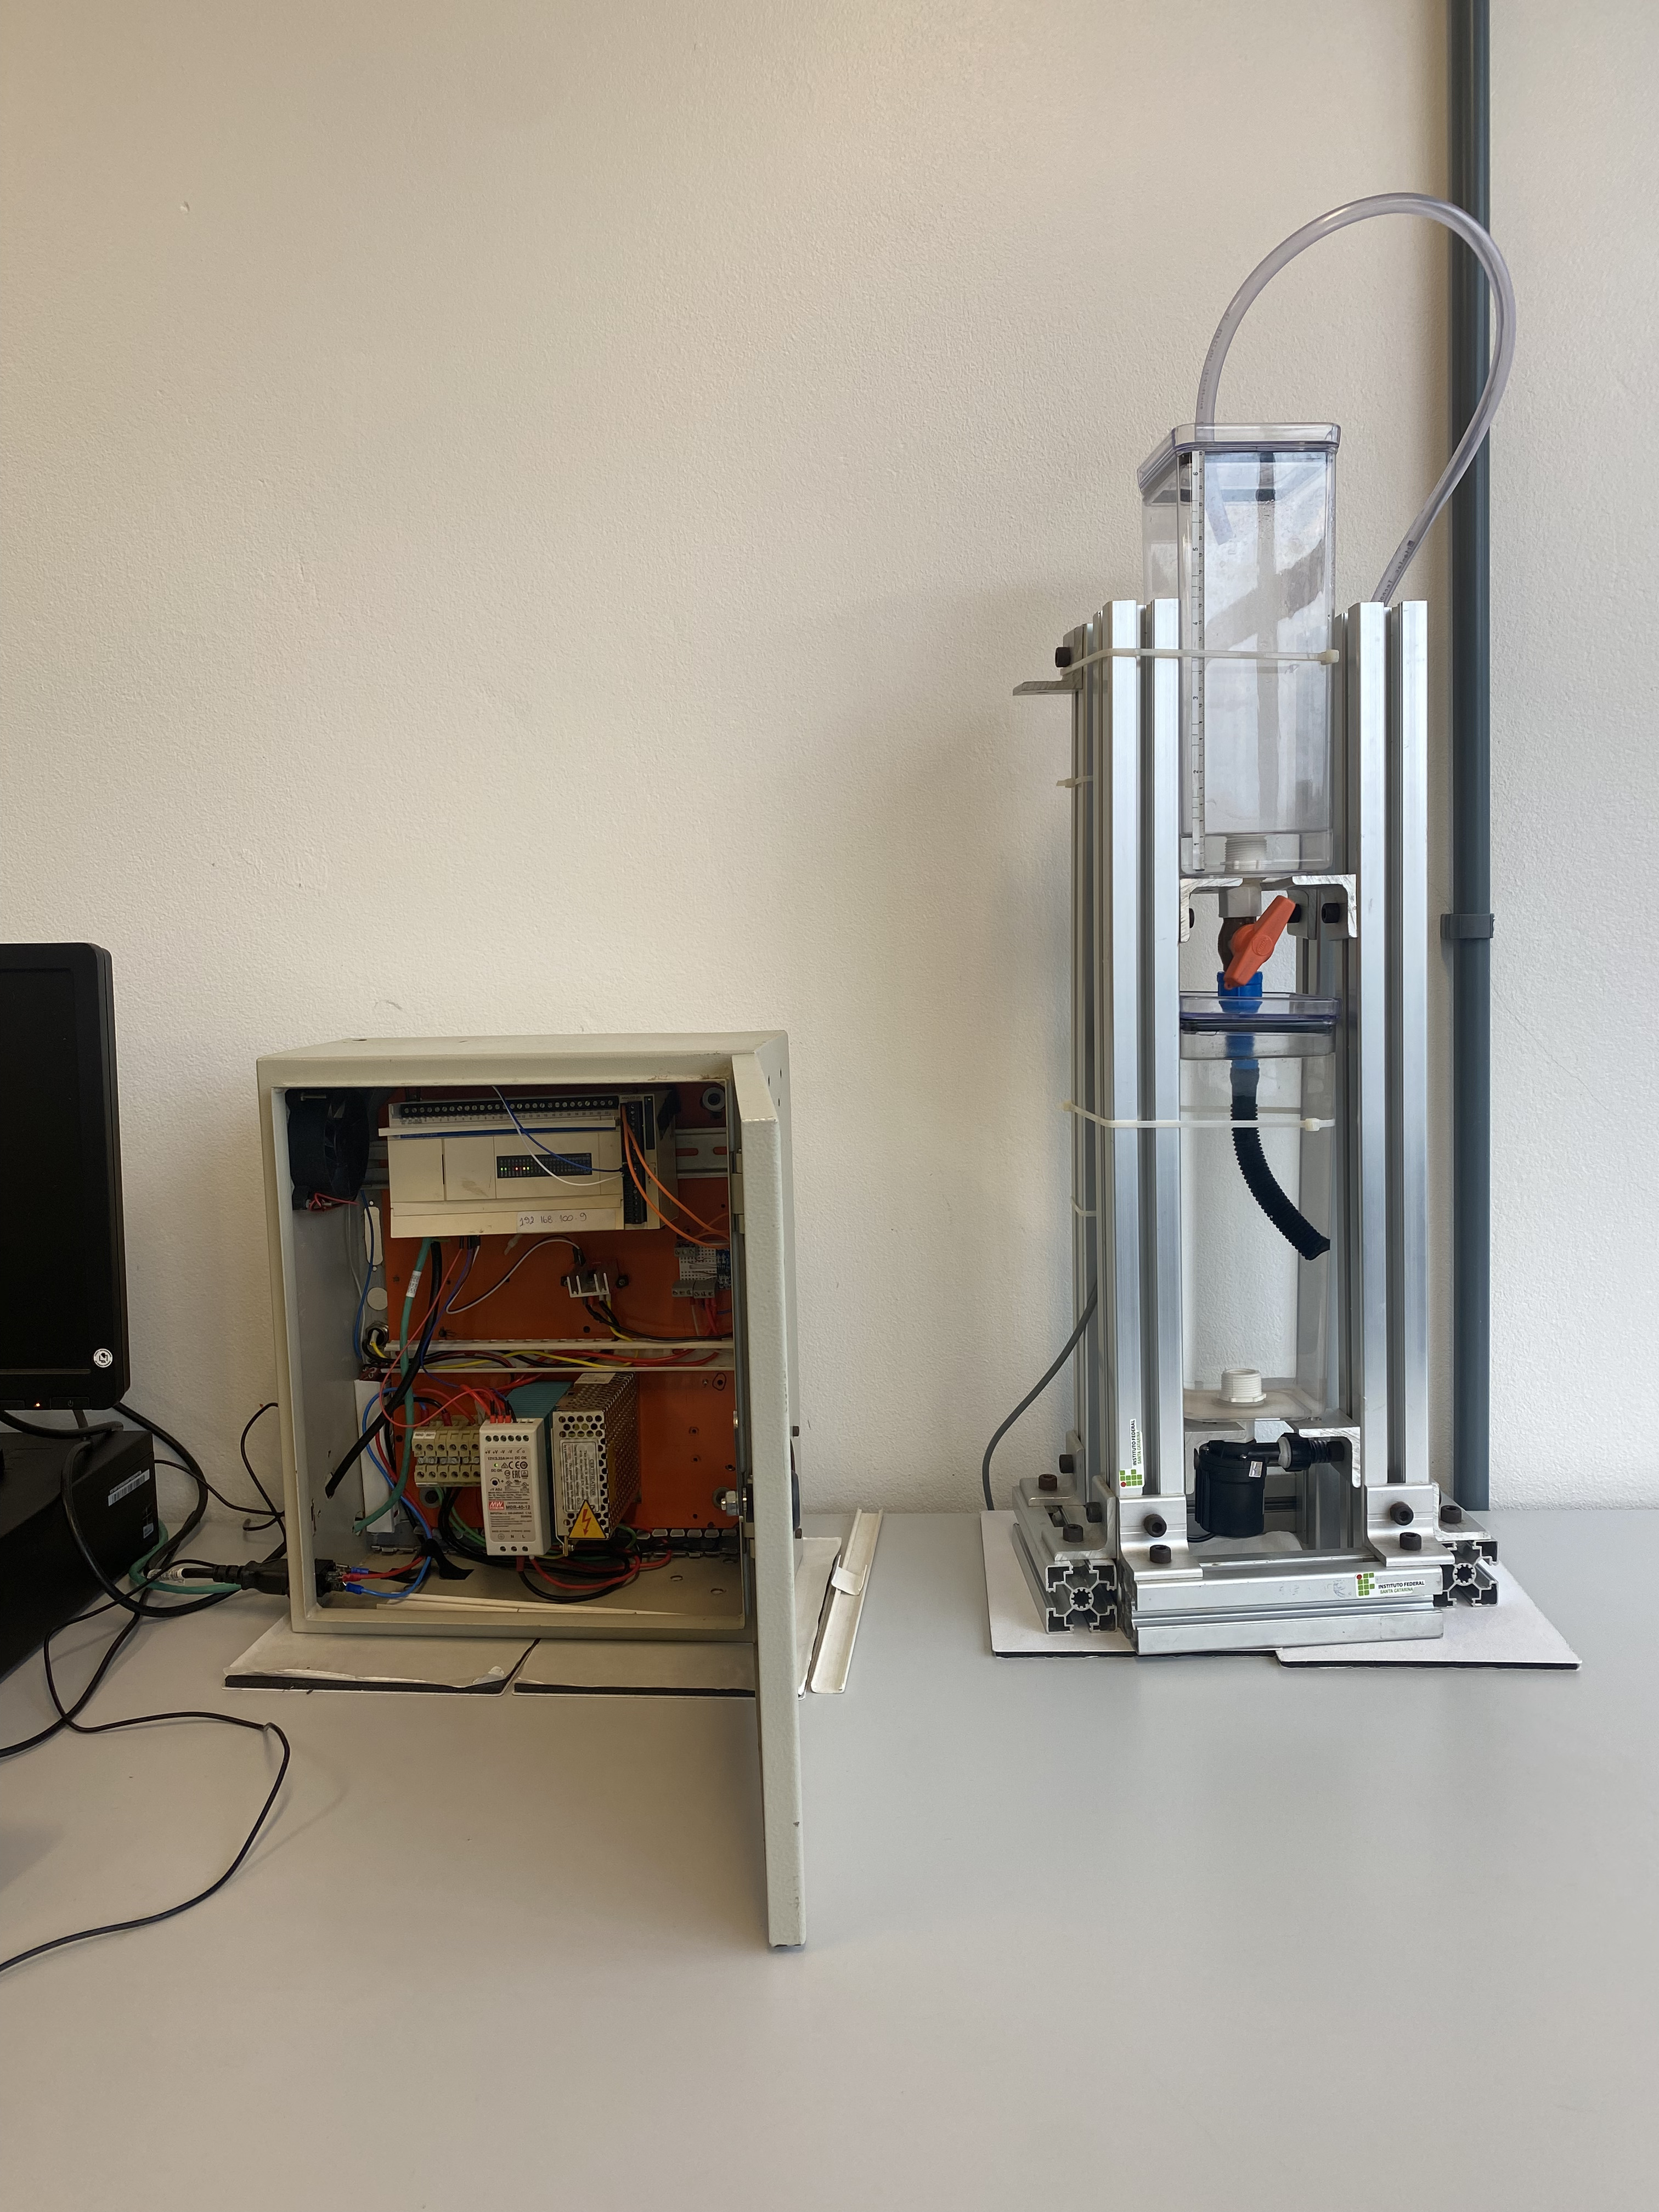
\includegraphics[scale=0.1]{imagens/sistema_geral.jpg}
    \end{center}
    \label{fig:esq}
    \par Fonte: Dos autores
\end{figure}

\subsection{Sistema controlado}
\hspace{11mm}O sistema apresenta dois tanques, montados um sobre o outro, fixados por perfis de alumínio e também apresenta uma interligação sobre eles controlada por um registro manual. Além disso, contém um atuador, um sensor de pressão e válvulas de entrada e saída.

A bomba, que pode ser vista na imagem \ref{fig:tanque_inf}, é o unico atuador do projeto e está interligando o tanque inferior a uma manqueira de retroalimentação ao tanque superior. O atuador utilizado tem uma potência de 19W e uma tensão de alimentação de 12V.

\begin{figure}[H]
        \centering\footnotesize
        \caption{Tanque inferior, com bomba acoplada}
        \begin{center}
            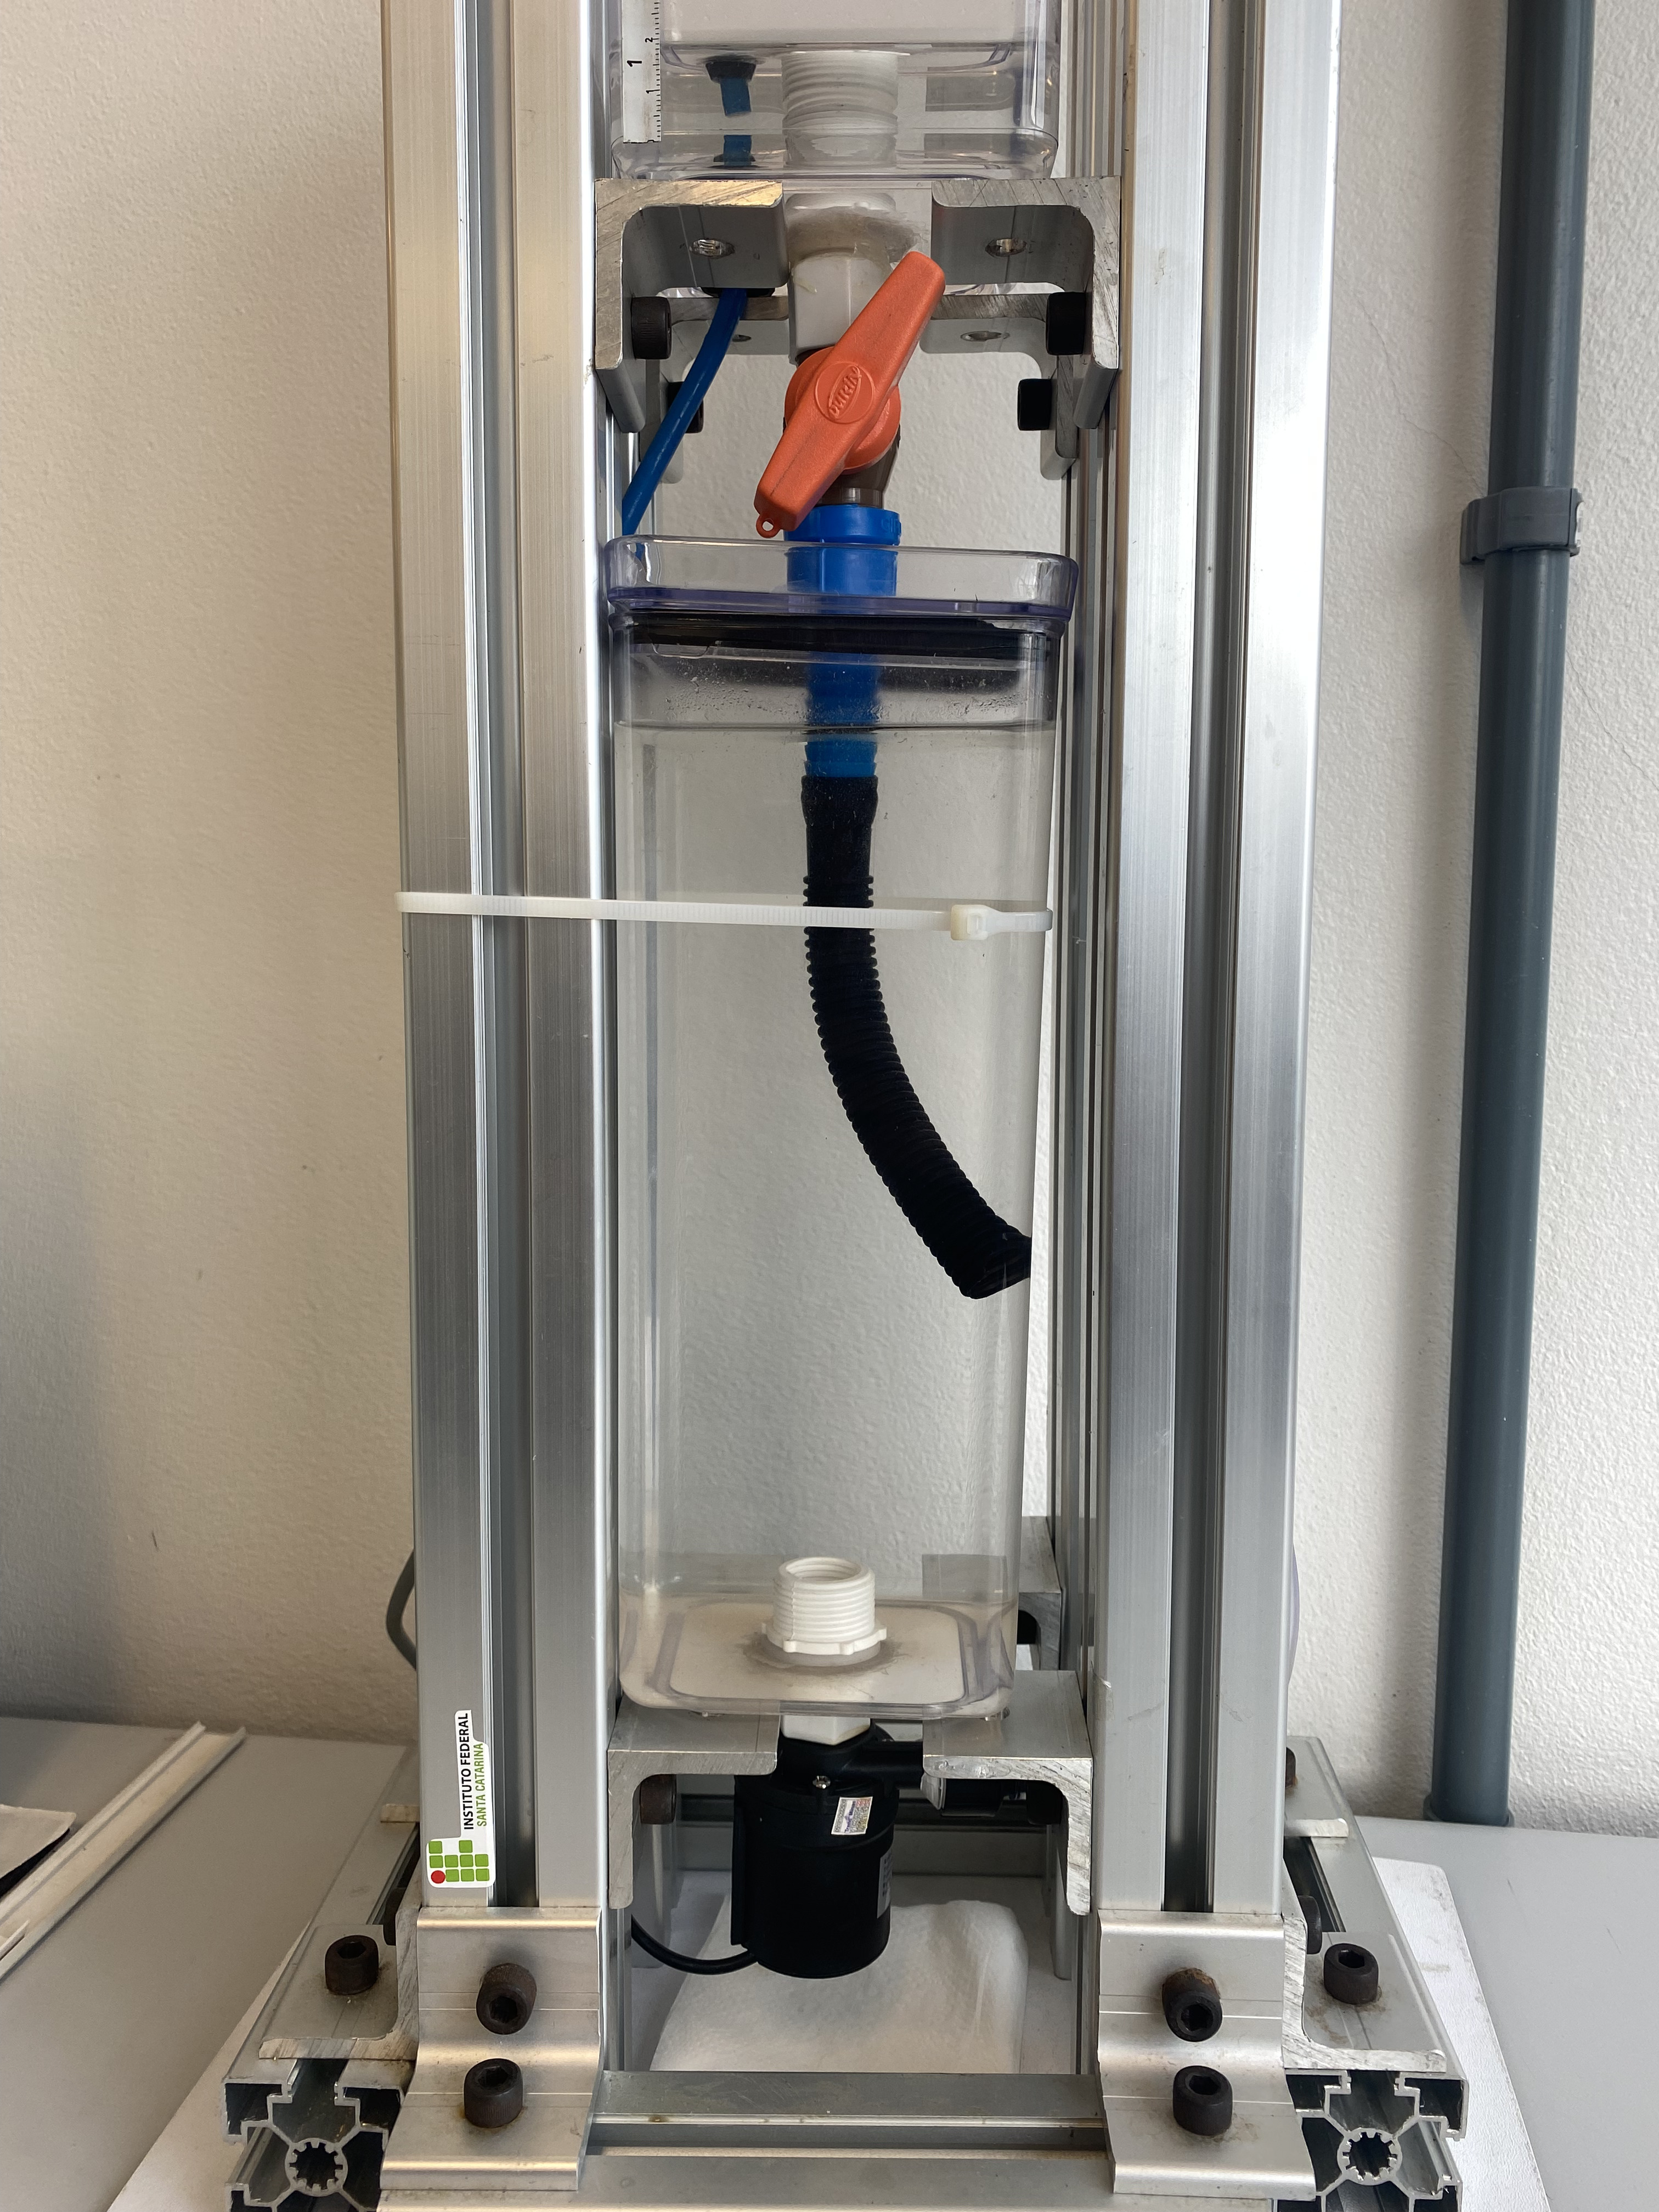
\includegraphics[scale=0.1]{imagens/tanque_inferior.jpg}
        \end{center}
        \label{fig:tanque_inf}
        \par Fonte: Dos autores
    \end{figure}

O sensor utilizado é um MPX2010DP, podendo ser visualizado na imagem \ref{fig:sensor}, é um sensor diferencial de pressão, o qual mede a diferença de pressão em dois pontos. Nesta planta, uma das aberturas do sensor está na pressão atmosférica e a outra no fundo do tanque superior, portando está sendo medido a pressão manométrica que a água exerce no sensor. Outro ponto importante a ser ressaltado, é de o sensor ter sido projetado para medir até 10KPa de pressão, pressão esta que tem magnitude superior que o sensor será submetido neste projeto, portanto foi acoplado um amplificador em sua saída, o qual será explicado melhor mais adiante.

\begin{figure}[H]
        \centering\footnotesize
        \caption{Sensor MPX2010DP acoplado ao tanque superior}
        \begin{center}
            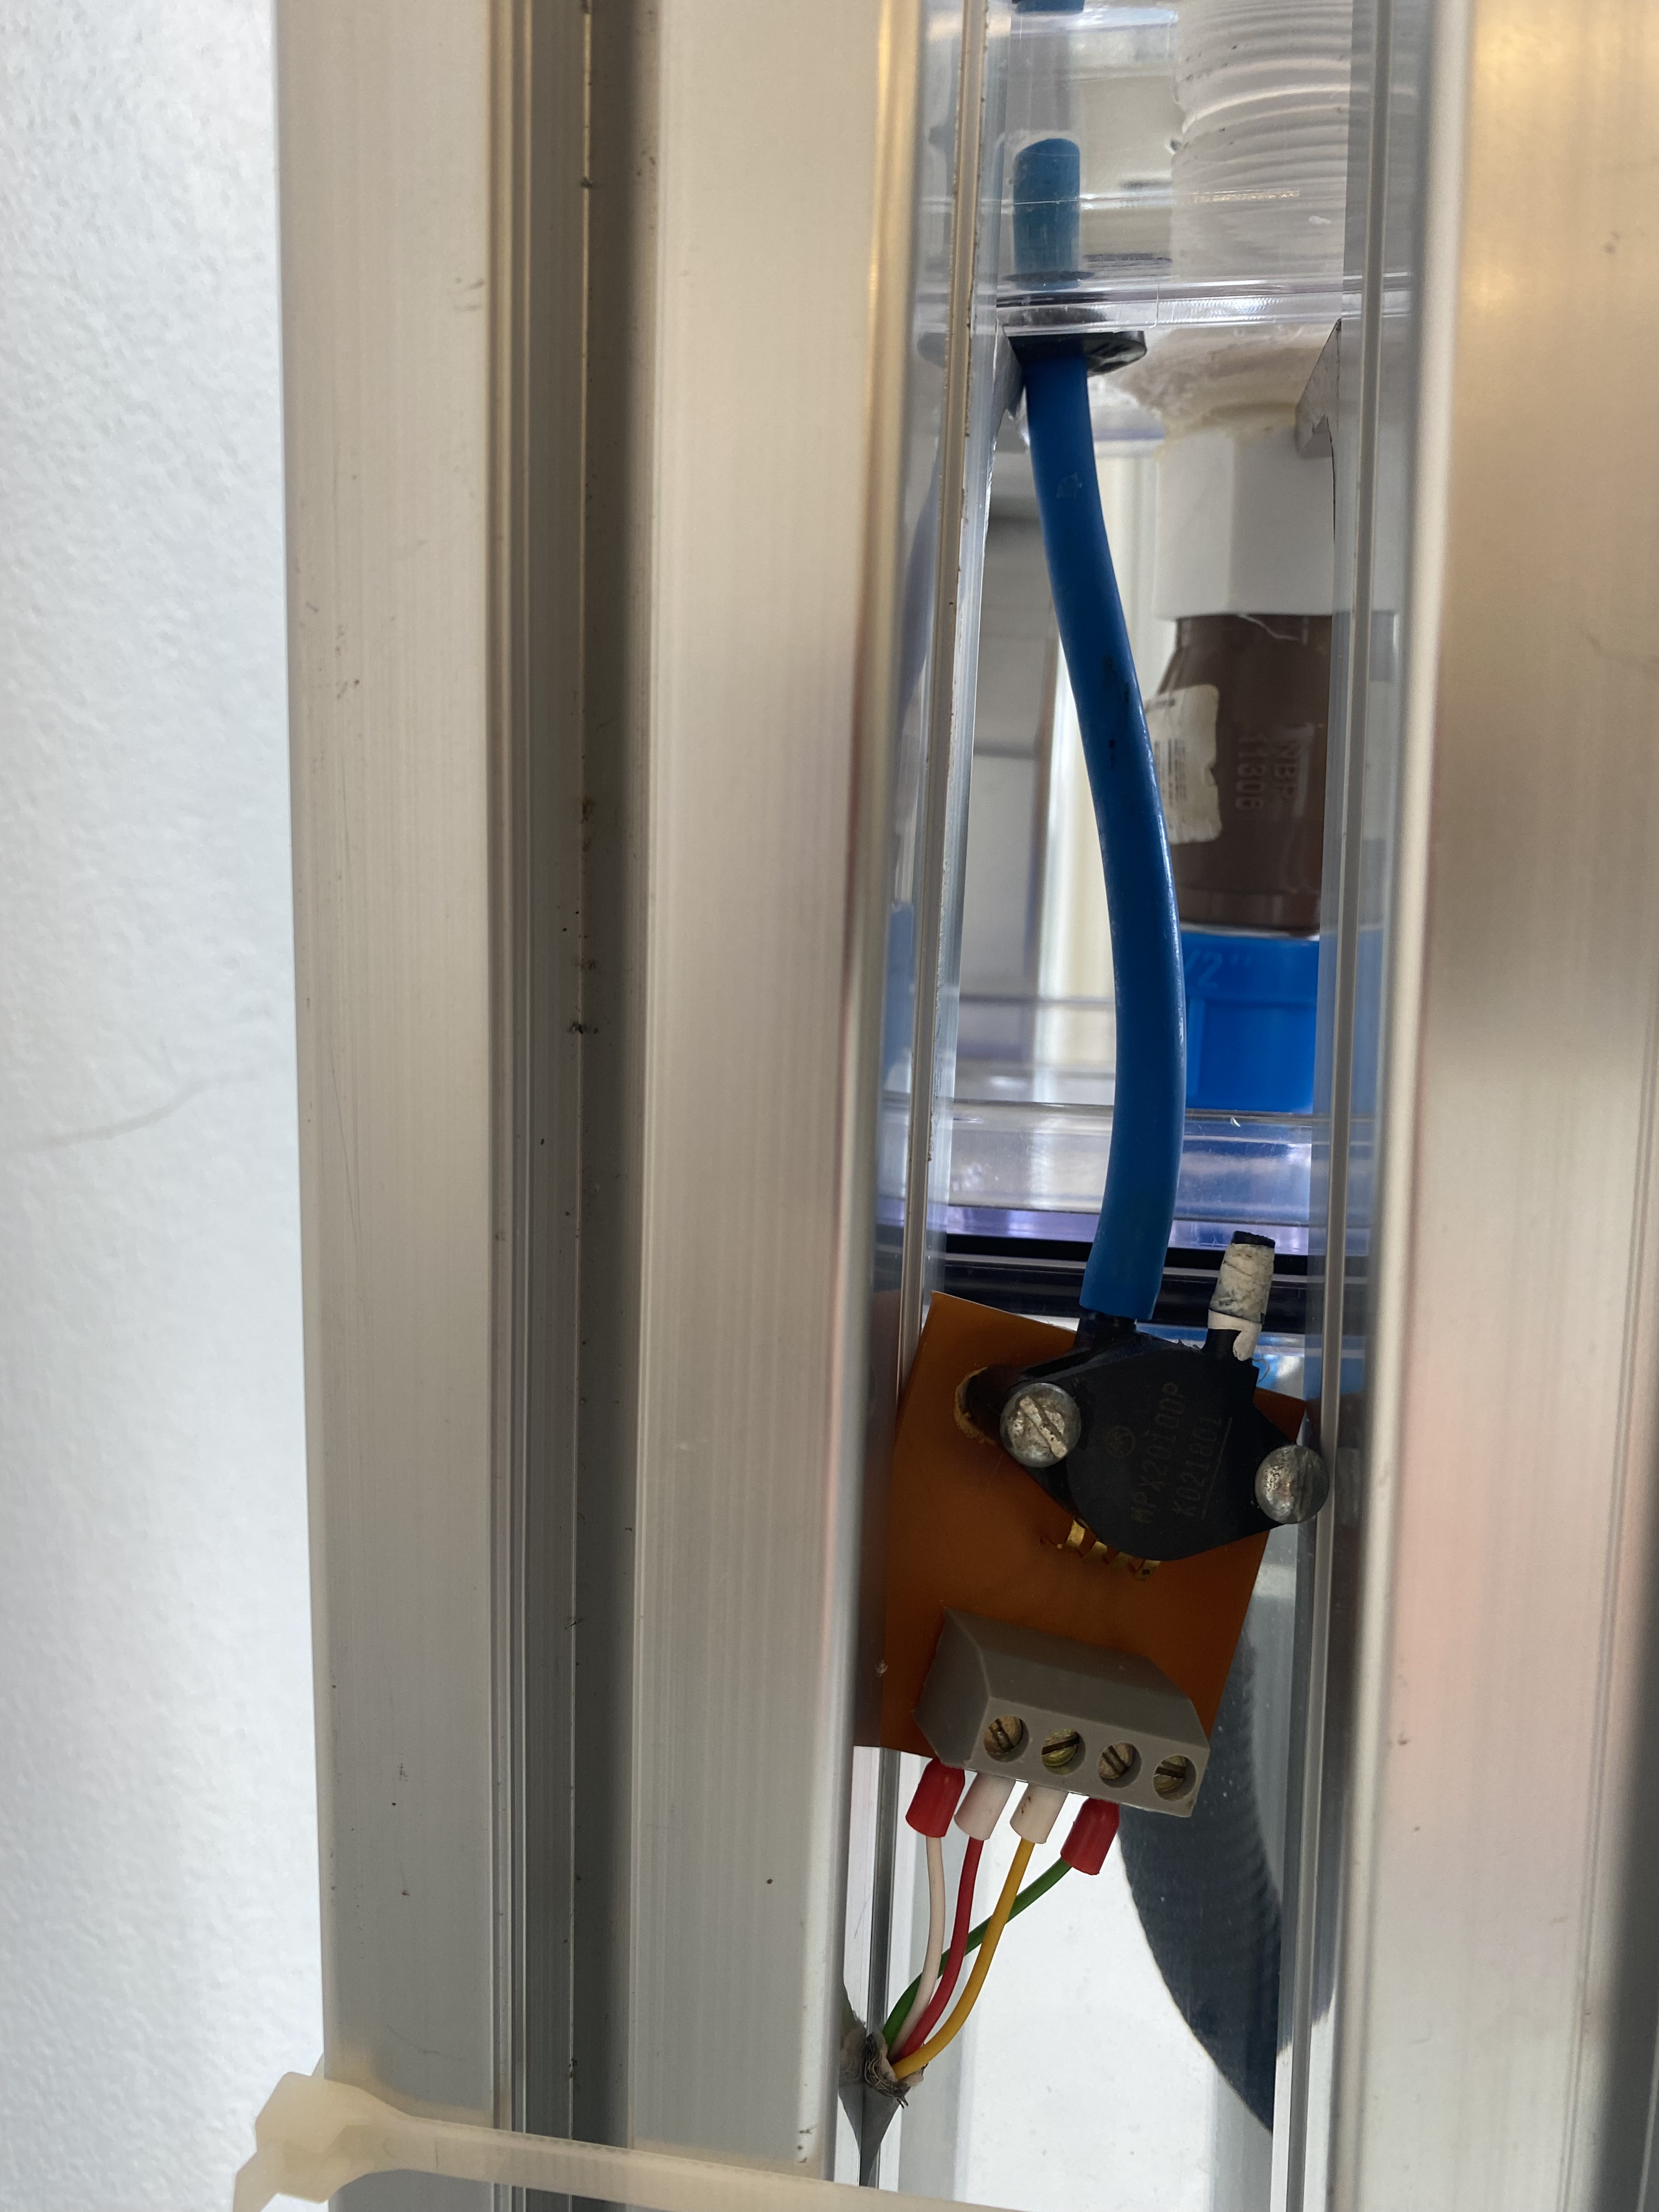
\includegraphics[scale=0.1]{imagens/sensor.jpg}
        \end{center}
        \label{fig:sensor}
        \par Fonte: Dos autores
    \end{figure}
    
Os tanques utilizados são feitos em acrílico, tendo aproximadamente ${100cm^2}$ de área de seção transversal e 25cm de altura, podendo ser visualizado o tanque superior na imagem \ref{fig:tanque_sup}.

\begin{figure}[H]
        \centering\footnotesize
        \caption{Tanque superior}
        \begin{center}
            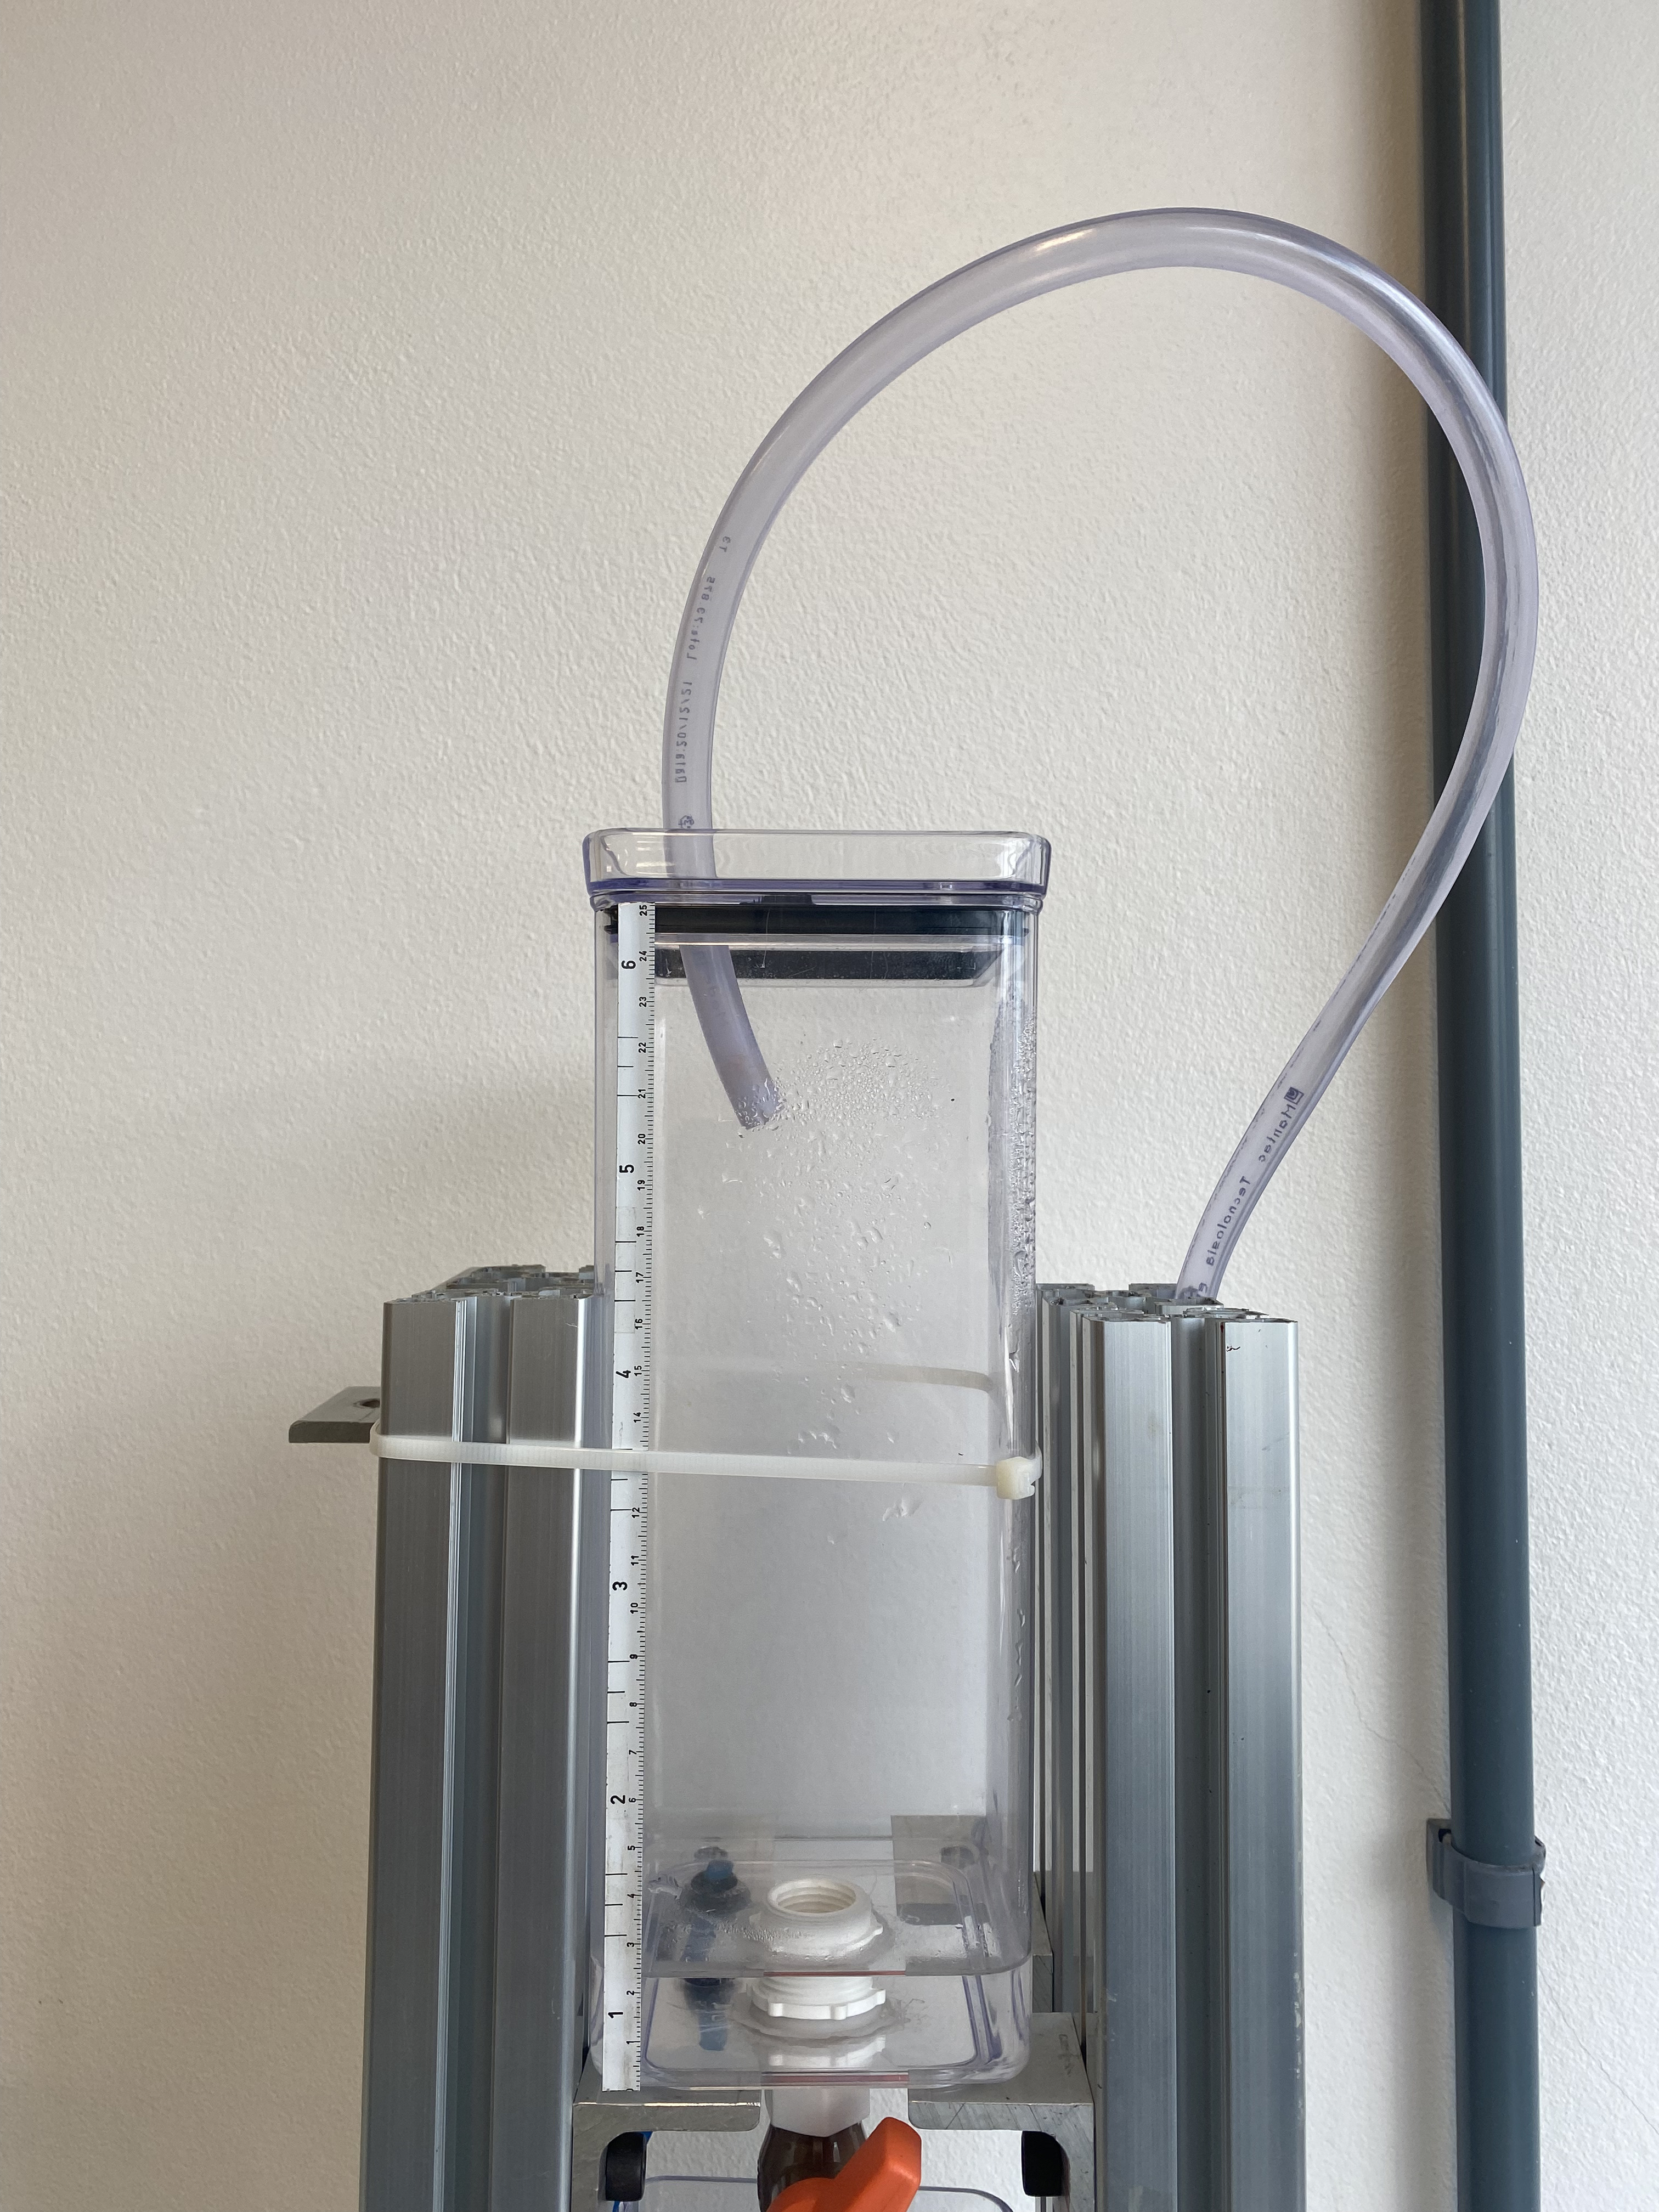
\includegraphics[scale=0.1]{imagens/tanque_superior.jpg}
        \end{center}
        \label{fig:tanque_sup}
        \par Fonte: Dos autores
    \end{figure}
    
\subsection{Painel de controle}
\hspace{11mm}O painel de controle é formado por um painel metálico que é utilizado para fixação de componentes para o controle da planta. Neste projeto encontra-se instalado no painel um Controlador Lógico Programavel (CLP), um amplificador de tensão, um driver DCIPF520, duas fontes de tensão, uma de 24V e uma de 12V. Na figura \ref{fig:painel} pode ser visualizada a disposição dos intens citados


\begin{figure}[H]
    \centering\footnotesize
    \caption{Painel de controle da planta}
    \begin{center}
        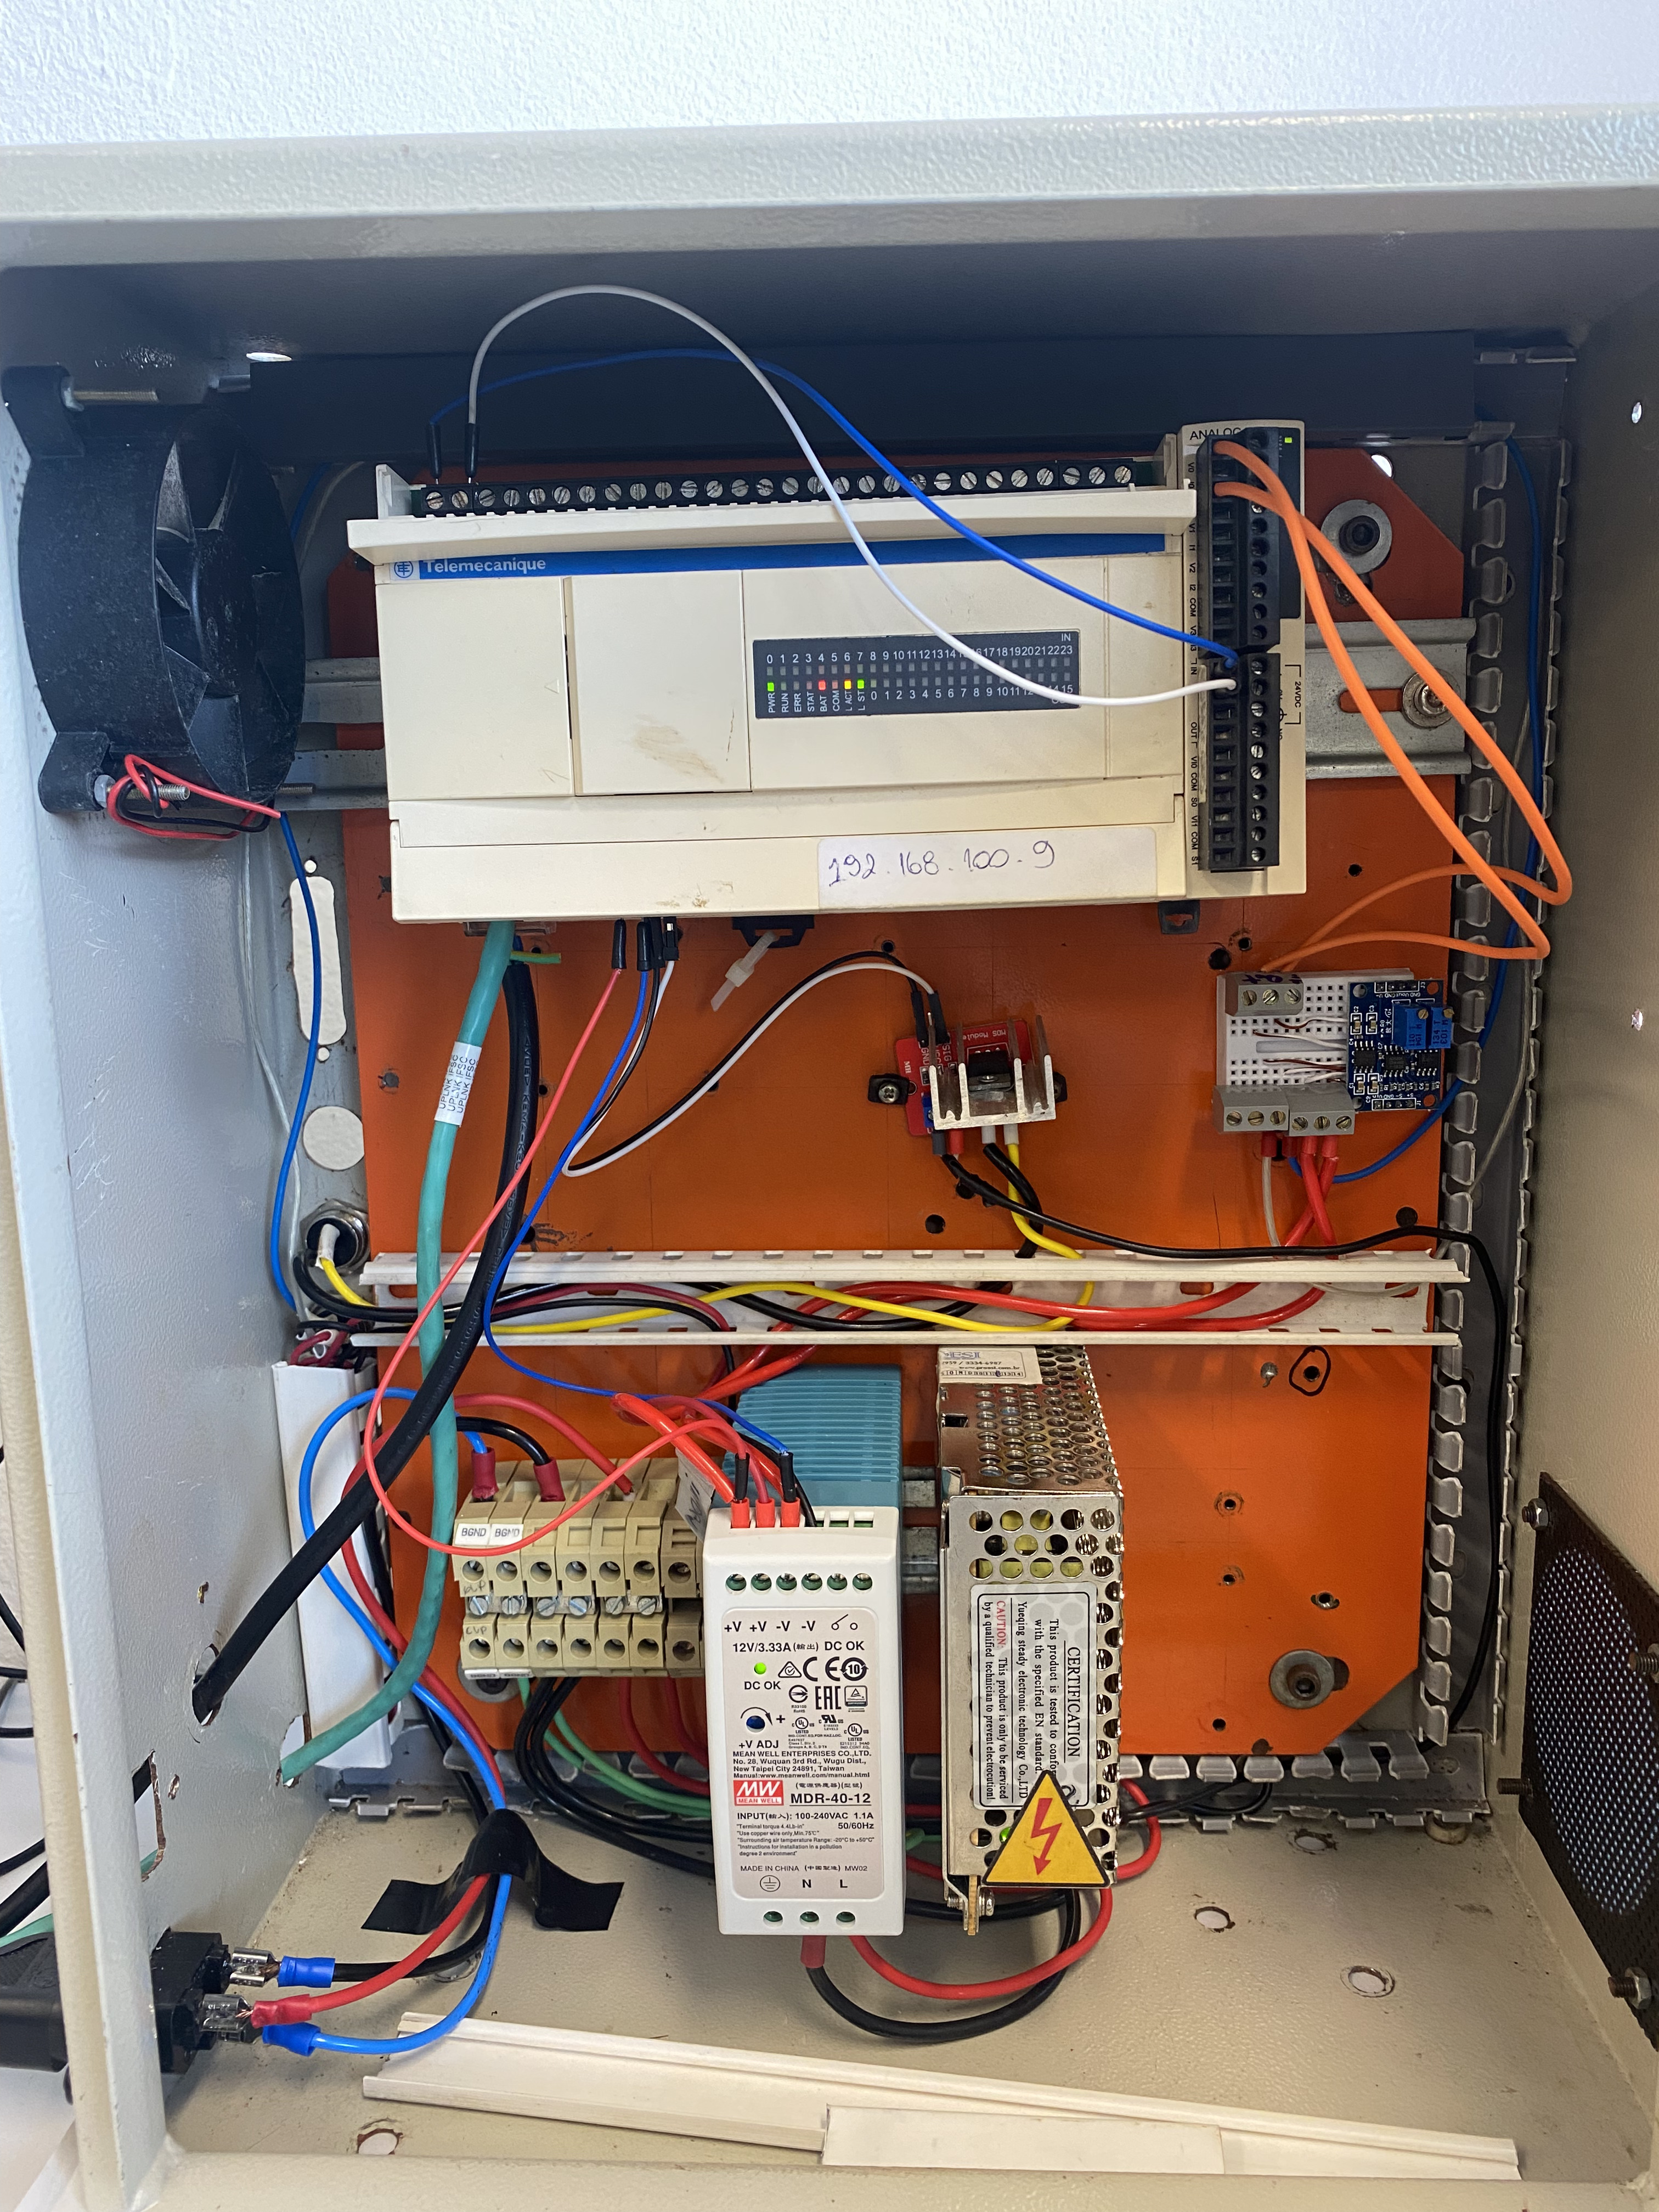
\includegraphics[scale=0.1]{imagens/painel.jpg}
    \end{center}
    \label{fig:painel}
    \par Fonte: Dos autores
\end{figure}
    
O CLP utilizado é fabricado pela Schneider Eletrics, é um Twido compact de modelo TWDLCAE40DRF, que está acoplado a um módulo com entradas analógicas para leitura do sensor e controle por PWM do driver da bomba. Podendo ser visualizado na imagem \ref{fig:clp}, este é o controlador que será utilizado para a implementação da lógica de controle de malha fechada.

\begin{figure}[H]
    \centering\footnotesize
    \caption{Twido}
    \begin{center}
        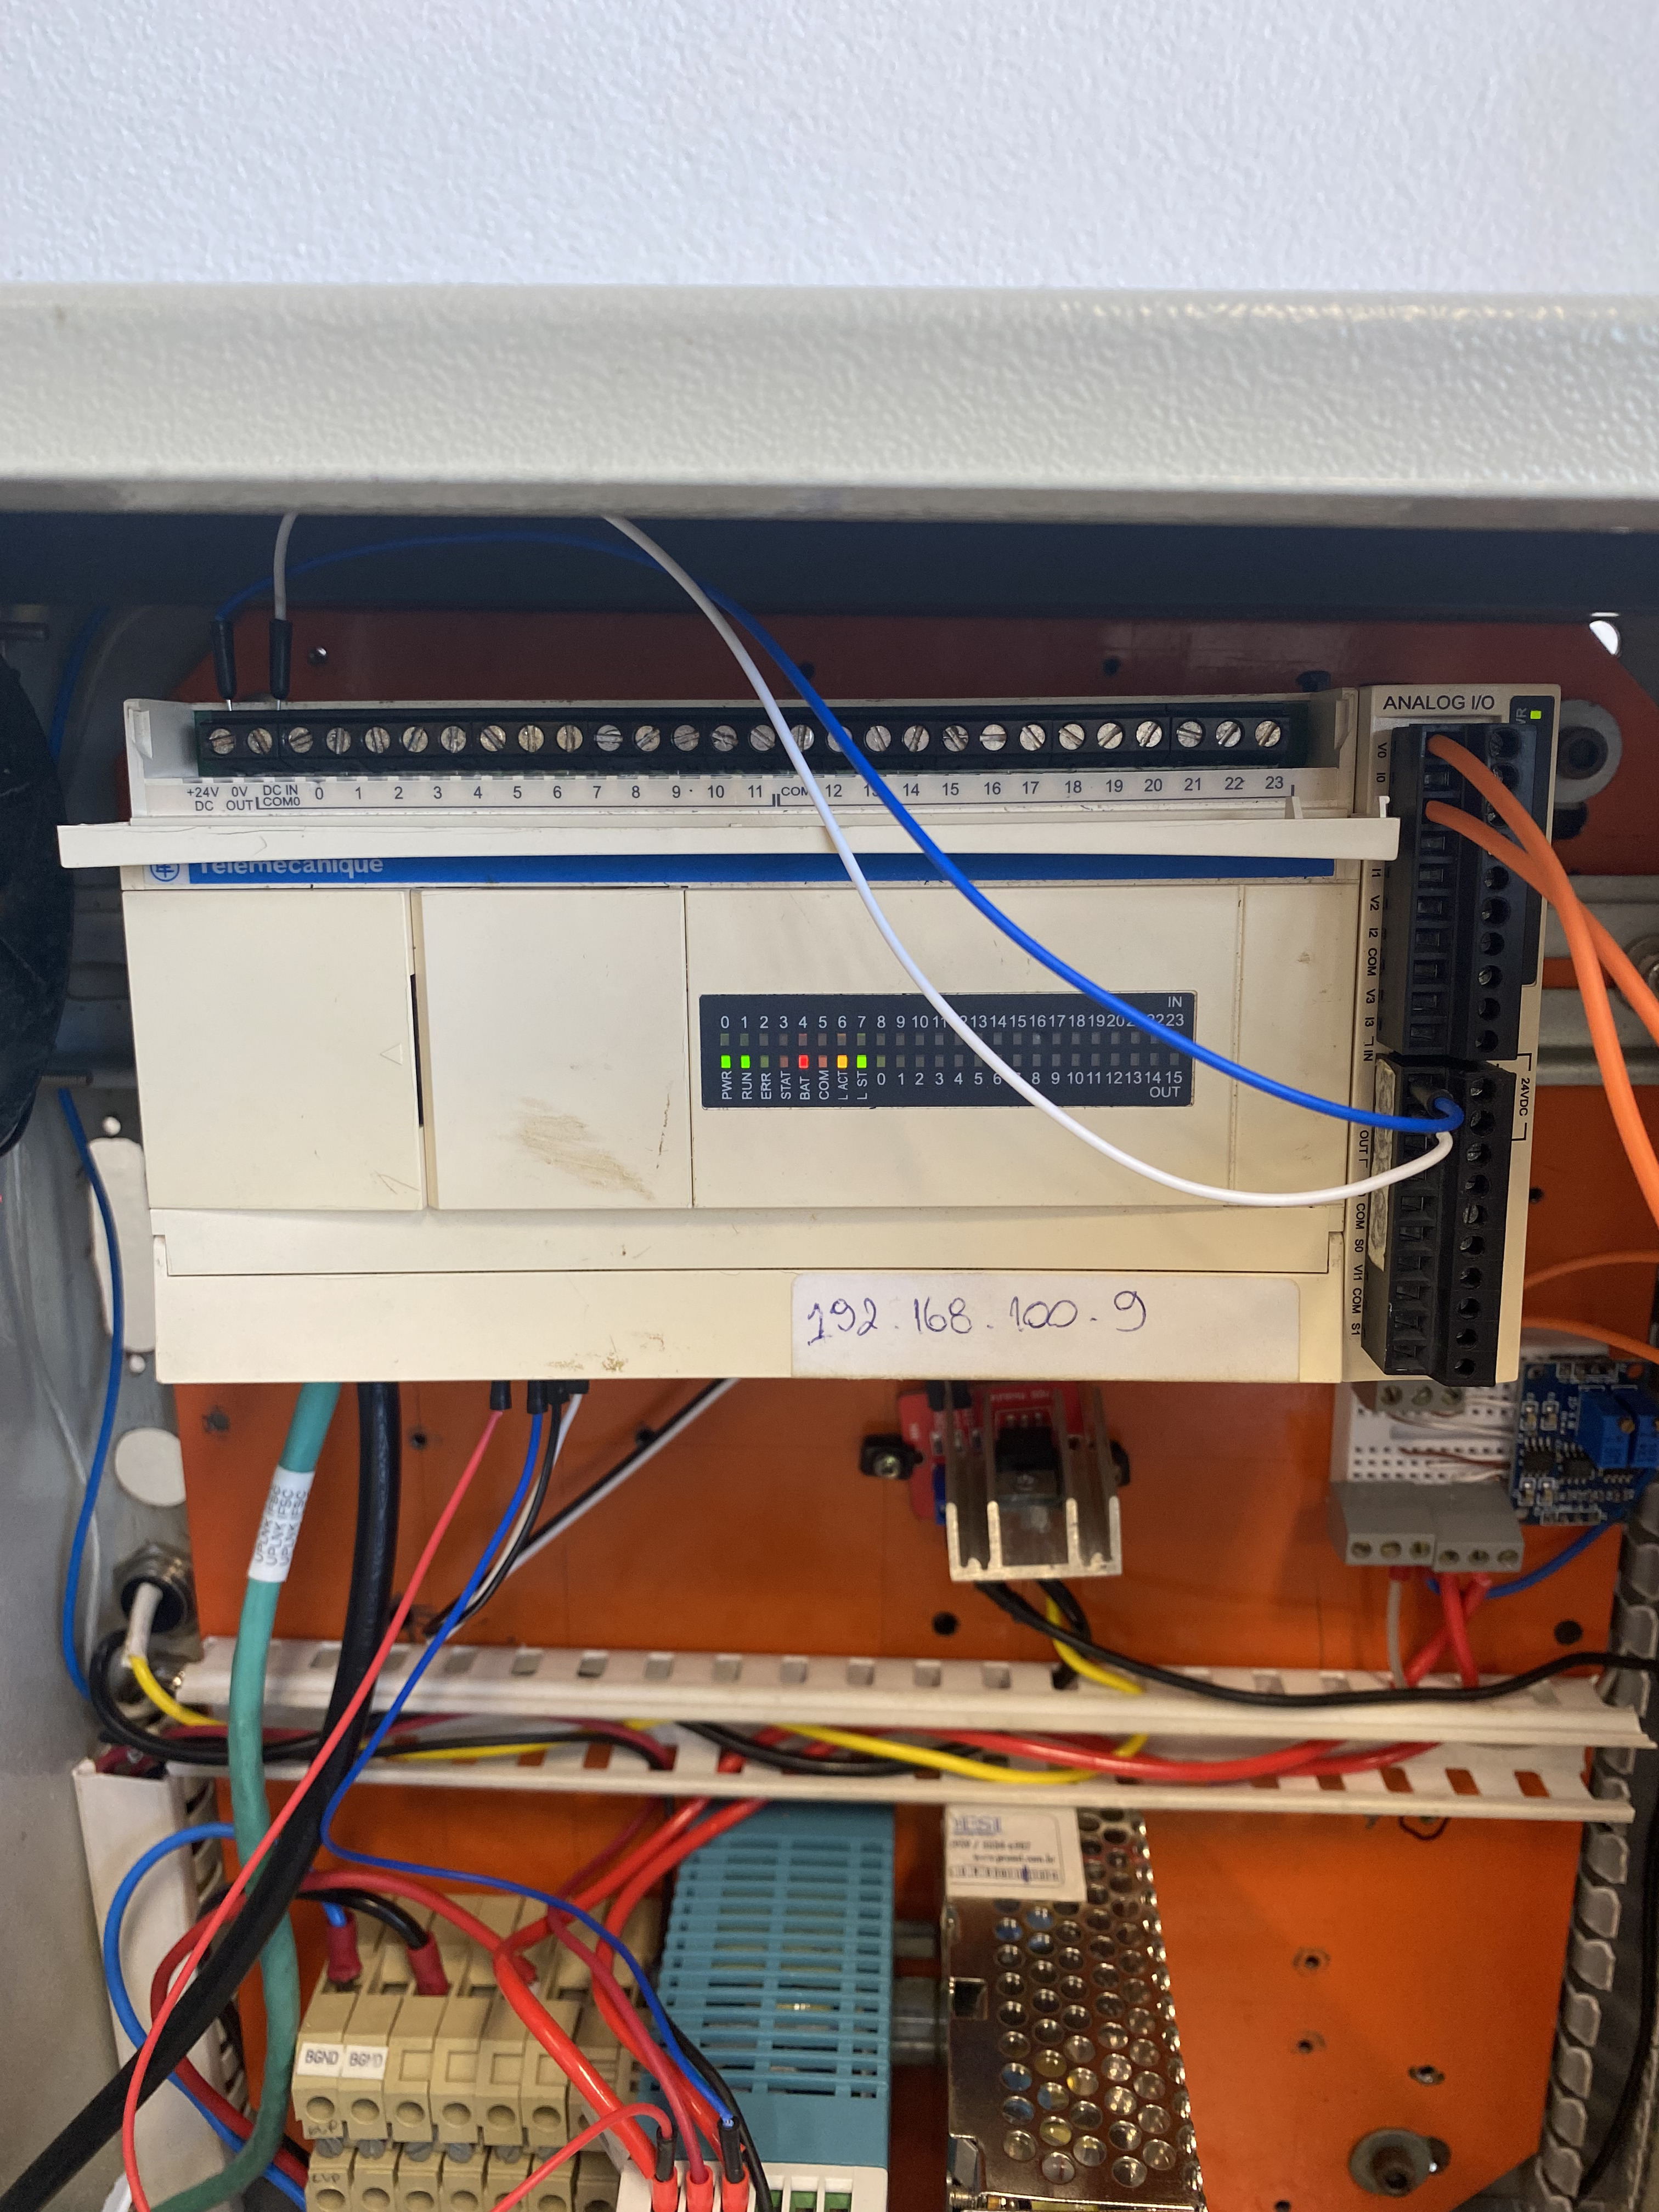
\includegraphics[scale=0.1]{imagens/clp.jpg}
    \end{center}
    \label{fig:clp}
    \par Fonte: Dos autores
\end{figure}

Para o controle do atuador, o sinal que sai do Controlador deve passar por um driver que faz o acionamento da bomba de acordo com o sinal enviado, em nosso projeto o driver DC-IRF520, observado na figura \ref{fig:driver}, tem uma tensão de trabalho de 3.3V a 5V e uma saída de até 24V.

\begin{figure}[H]
    \centering\footnotesize
    \caption{DC-IRF520}
    \begin{center}
        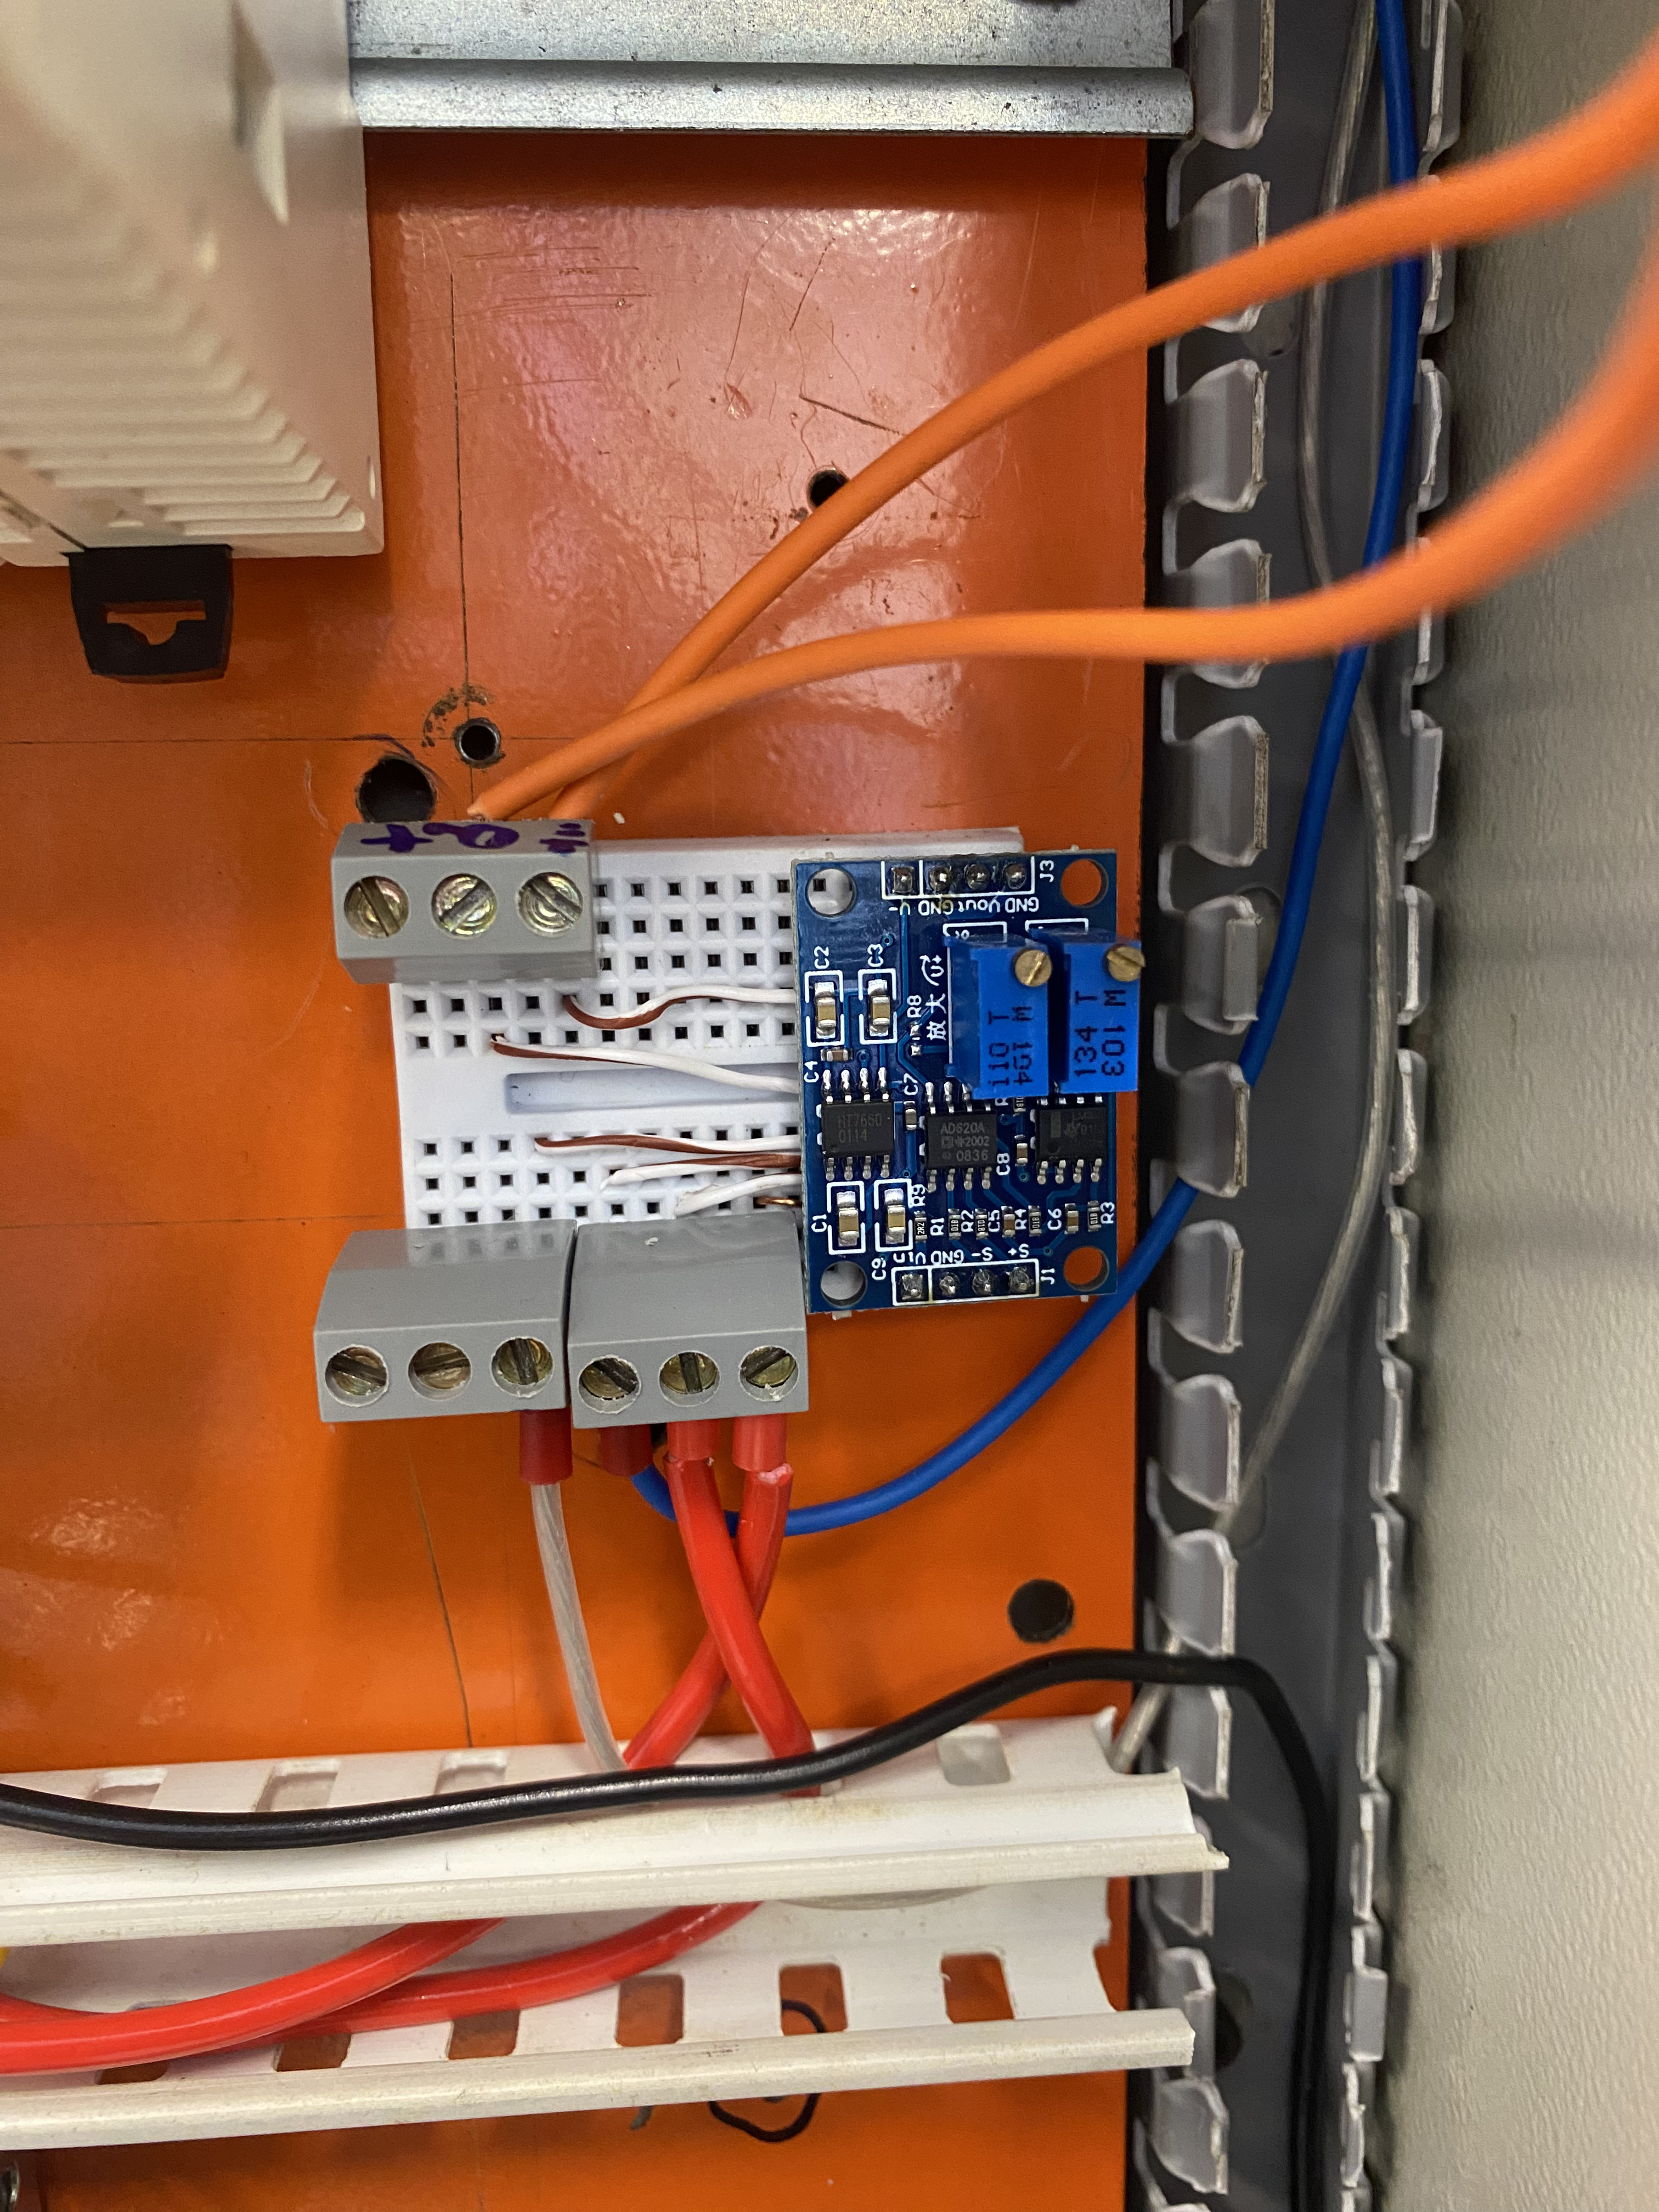
\includegraphics[scale=0.1]{imagens/amplificador.jpg}
    \end{center}
    \label{fig:driver}
    \par Fonte: Dos autores
\end{figure}

Na saída do sensor foi utilizado um Amplificador de tensão, para aumentar o sinal enviado pelo transdutor de pressão. O amplificador do sistema é do modelo AD620, possuindo uma ampliação ajustável de até 1000 vezes e uma tensão de trabalho de 3V a 12V e uma tensão de entrada que pode variar de 100$\mu$V ateé 300mV. O amplificador pode ser visualizado na imagem abaixo:

\begin{figure}[H]
    \centering\footnotesize
    \caption{Amplificador de sinal}
    \begin{center}
        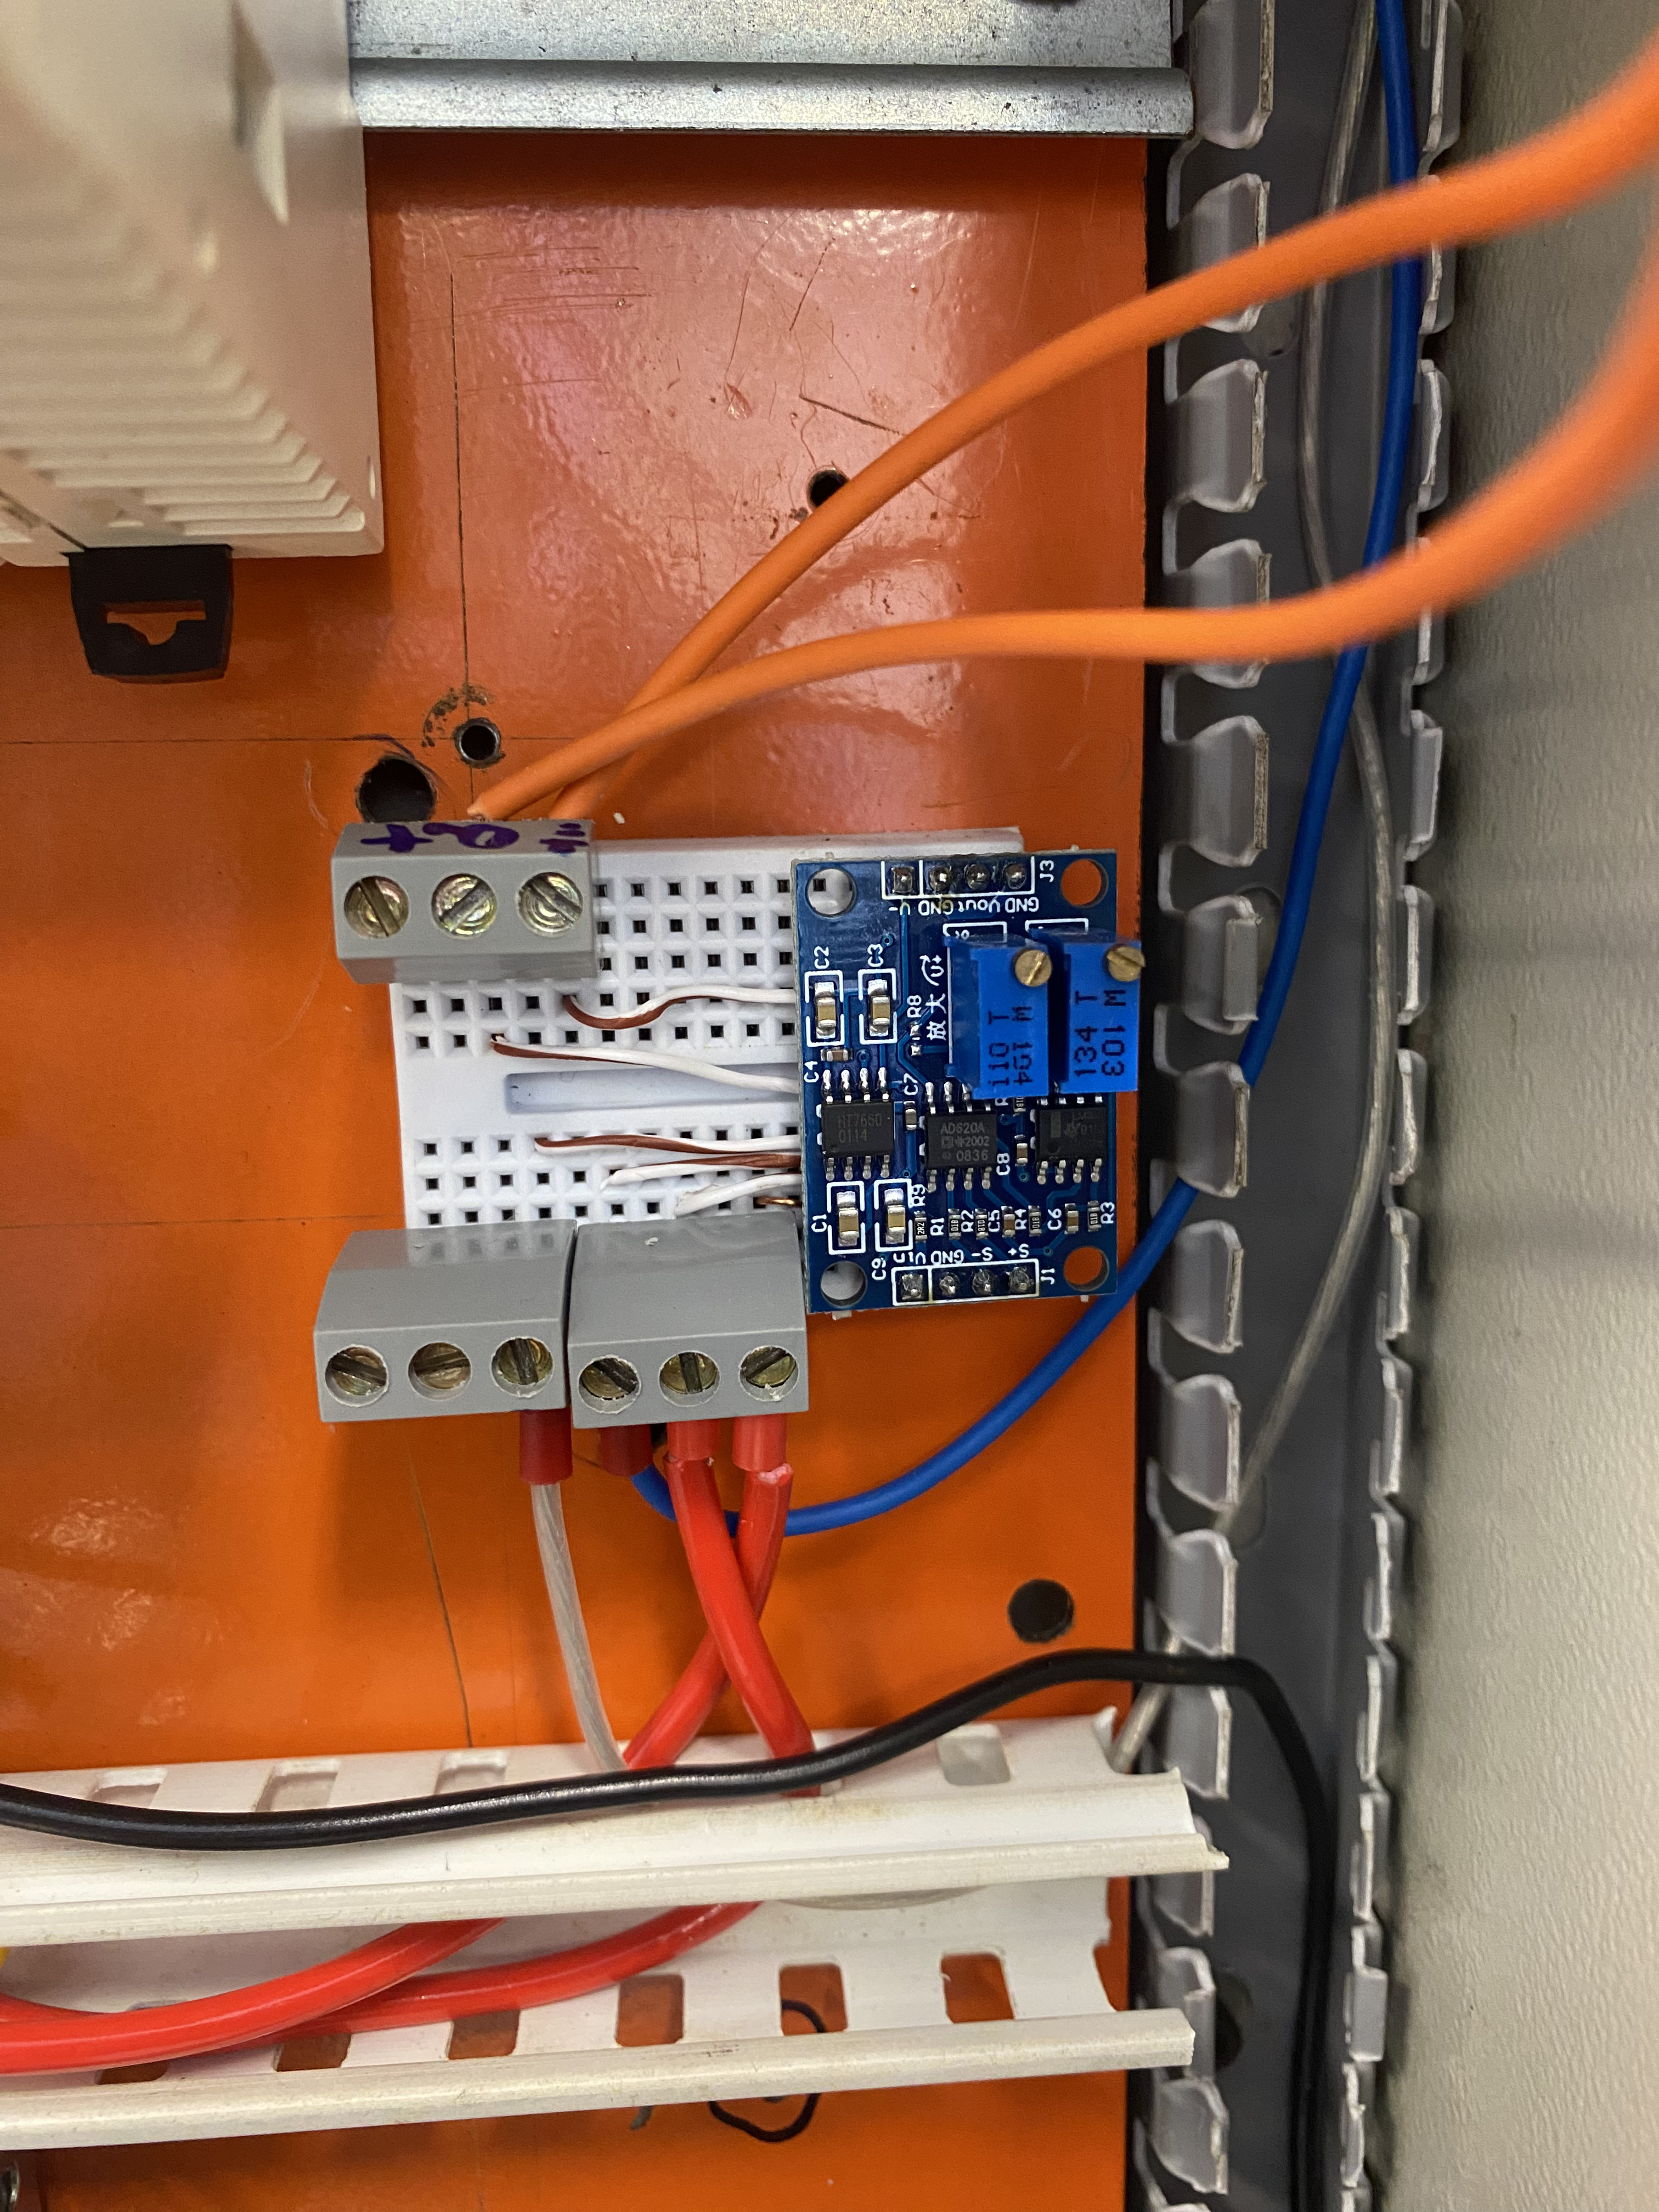
\includegraphics[scale=0.1]{imagens/amplificador.jpg}
    \end{center}
    \label{fig:amp}
    \par Fonte: Dos autores
\end{figure}


Além disso, foram utilizadas duas fontes chaveadas, uma com tensão de saída de 12V e uma de 24V que foram utilizadas para alimentar o sistema com as tensões e correntes necessárias para o funcionamento do sistema. As fontes podem ser observadas na imagem \ref{fig:fonte}.

\begin{figure}[H]
    \centering\footnotesize
    \caption{fontes}
    \begin{center}
        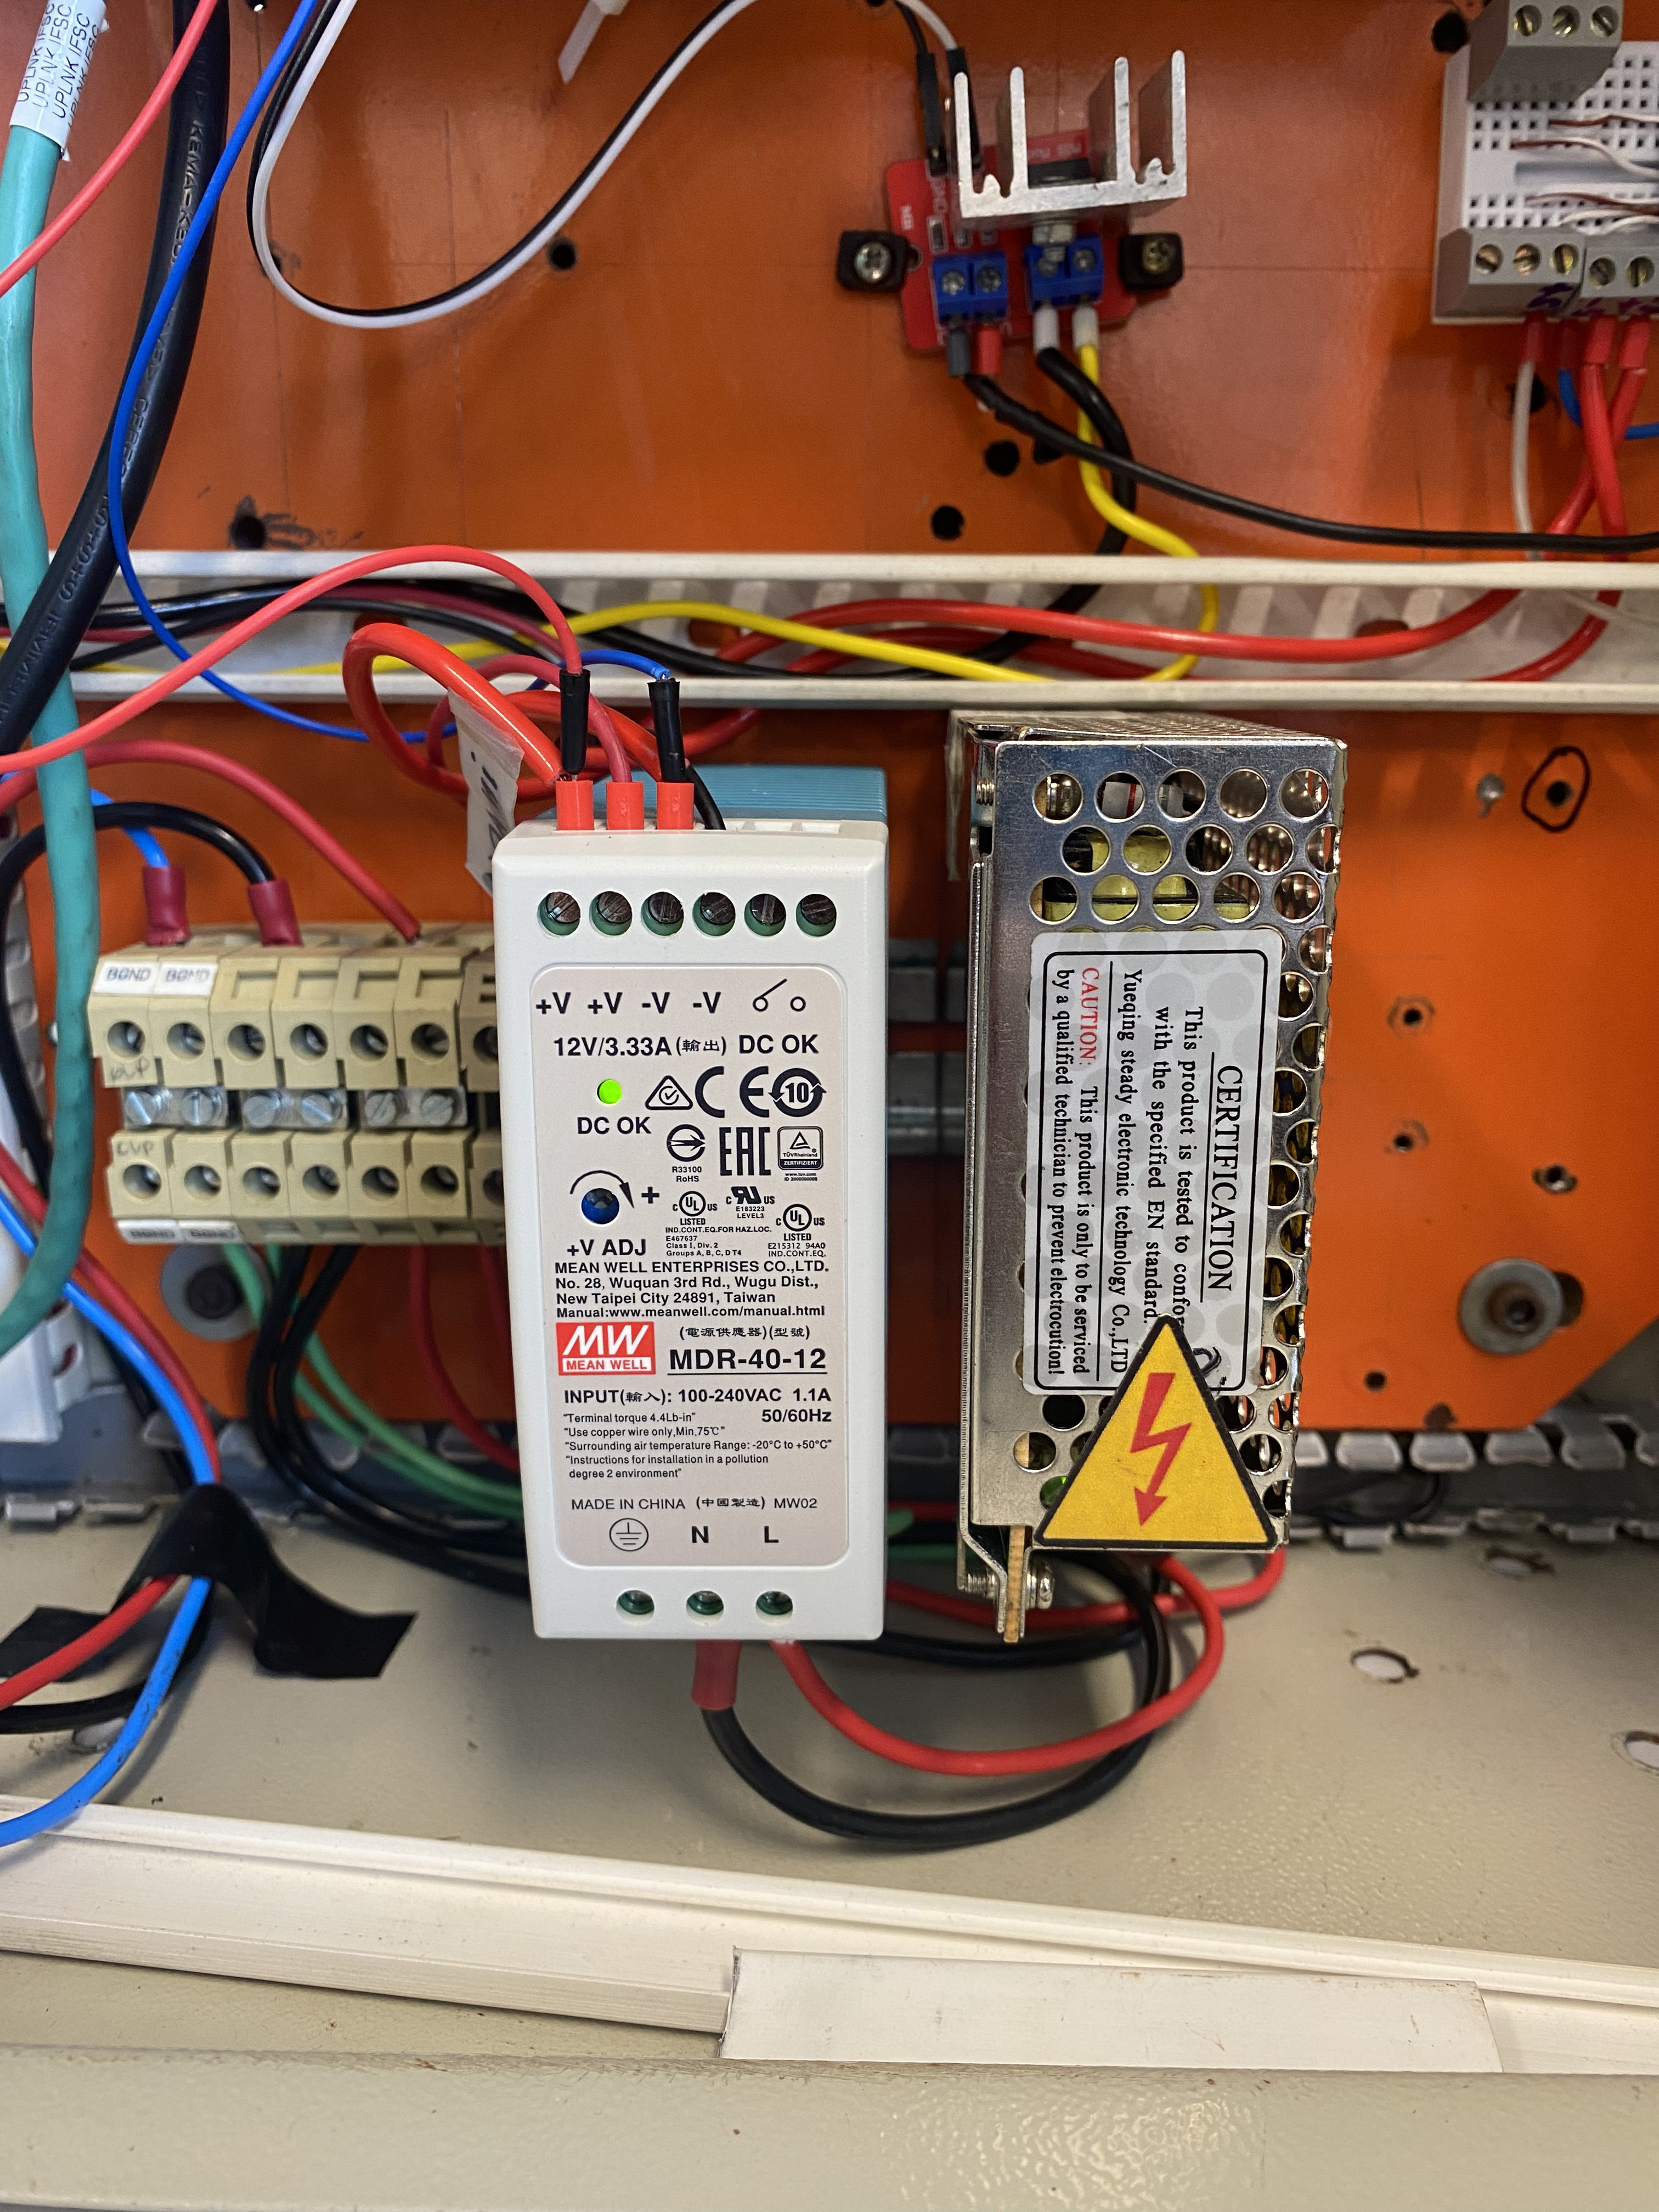
\includegraphics[scale=0.1]{imagens/fontes.jpg}
    \end{center}
    \label{fig:fonte}
    \par Fonte: Dos autores
\end{figure}

\section{Metodologia de identificação do sistema em malha aberta}
\hspace{11mm} Para identificação do sistema em malha aberta, primeiramente foi estimado o modelo matemático da planta a partir das equações teóricas que caracterizam a planta. Em um segundo momento, aproximou-se o modelo matemático da planta de forma empírica com o método de Smith.

\subsection{Identificação Teórica}

Neste processo foi criado um modelo matemático da planta, com algumas simplificações, para que pudessem ser encontradas as funções transfêrencias de algumas faixas de trabalho do sistema. Além disso, foi necessário alguns experimentos práticos para se determinar o valor de algumas variáveis necessárias para a solução das equações.

\subsubsection{Equacionamento das características}

Considerando o objetivo de controle do nível a partir da altura (h), o equacionamento foi iniciado a partir da lei de conservação da massa, com ela podemos inferir que a variação do volume deve ser igual a vazão de entrada menos a vazão de saída: 

\begin{equation}
    \dfrac{dV}{dt} = V_e - V_s
\end{equation}
Como a área de seção transversal do tanque é aproximadamente constante, podemos dizer que:


\begin{equation}
    \dfrac{dV}{dt} = dh \cdot \dfrac{A}{dt}
\end{equation}

Assim, foi obtida a equação que relaciona a altura (h) a variação da vazão, Ve-Vs:


\begin{equation}
    \dfrac{dh}{dt} = \dfrac{V_e - V_s}{A}
\end{equation}

Estimou-se Ve, a vazão controlada pela bomba, como uma constante K multiplicado uma tensão média, vinda do driver da bomba:


\begin{equation}
    V_e = K \cdot U
\end{equation}

Foi reescrito Vs da seguinte forma:

\begin{equation}
    V_s = a \cdot v
\end{equation}

Onde "a" é a área efetiva da válvula de saída do tanque superior e "v" é a velocidade da água que está saindo do tanque. Utilizando-se Bernoulli, foi possivel escrever a vazão de saída do  tanque em função da área de saída da pressão e da massa específica da água, como visto na equação abaixo.

\begin{equation}
    V_s = a\cdot \sqrt{2g} \cdot \sqrt{\dfrac{P}{g \rho}}
\end{equation}

Sendo assim, foi obtida a seguinte equação:
\begin{equation}
    \dfrac{dh}{dt} = \dfrac{KU - a\cdot \sqrt{2g} \cdot \sqrt{h}}{A}
\end{equation}

E então foi feita a substituição de "h" e "U" por um valor de referência, "$h_0$" e "$U_0$", adicionados por um delta:

\begin{equation}
    h = \Delta h + h_0
\end{equation}
\begin{equation}
    U = \Delta U + U_0
\end{equation}
\begin{equation}
    \dfrac{d(\Delta h + h_0)}{dt} = \dfrac{K(\Delta U + U_0) - a\cdot \sqrt{2g} \cdot \sqrt{\Delta h + h_0}}{A}
\end{equation}

Em um estado de equilíbrio pode ser obtido:

\begin{equation}
    KU_0 = a\cdot \sqrt{2g} \cdot \sqrt{ h_0}
\end{equation}

Para que pudesse ser trabalhado com um sistema de primeira ordem, foi feita a linearização do termo $\sqrt{\Delta_h}$da penúltima equação, utilizando os primeiros dois termos da série de taylor, obtendo o seguinte resultado:

\begin{equation}
    \dfrac{d(A\cdot \Delta h)}{dt} = \Delta UK - \dfrac{a\cdot \sqrt{2g} \cdot \Delta h}{2 \cdot \sqrt{h_0}} + KU_0 - a \cdot \sqrt{2gh_0}
\end{equation}

É possível eliminar alguns termos, quando consideramos um estado de equilíbrio:

\begin{equation}
    \dfrac{d(\Delta h A)}{dt} = \Delta UK - \dfrac{a\cdot \sqrt{2g} \cdot \Delta h}{2 \cdot \sqrt{h_0}}
\end{equation}

Fazendo a substituição de alguma constantes e isolando $\Delta h$, tem-se que:

\begin{equation}
    \alpha = \dfrac{a\cdot \sqrt{2g} \cdot \Delta h}{2 \cdot \sqrt{h_0}}
\end{equation}
\begin{equation}
    \tau = \dfrac{A}{\alpha}
\end{equation}
\begin{equation}
    K_e = \dfrac{K}{\alpha}
\end{equation}
\begin{equation}
    \Delta h = \dfrac{\Delta U \cdot K_e}{s\cdot \tau + 1}
\end{equation}
\begin{equation}
    \dfrac{\Delta h}{\Delta U} = \dfrac{K_e}{\tau\cdot s + 1}
\end{equation}

\subsubsection{Analize e medição de constantes}
\hspace{11mm}Para calcular os valores da função de transferência obtida em 3.2.1.2, foi necessário medir e estimar os valores de algumas constantes da planta, sendo elas: a (área efetiva de abertura da válvula de saída do tanque), A (área de seção transversal do tanque) , a qual foi medida com um paquimetro, e K (constante que relaciona a tensão média na bomba com a vazão gerada) e h0 (alturas de referencia).

A constante K foram feitos ensaios com a válvula de saída do tanque fechada, e ativando a bomba em uma série de razões cíclicas de PWM por um tempo constante de 10s controlado pelo CLP em malha aberta. Multiplicando a diferença de altura pela área do tanque foi obtida a diferença de volume e dividindo a diferença pelo tempo decorrido, a vazão para aquele PWM. segue plotagem dos pontos:

\begin{figure}[H]
    \centering\footnotesize
    \caption{Gráfico para calculo da constante K}
    \begin{center}
        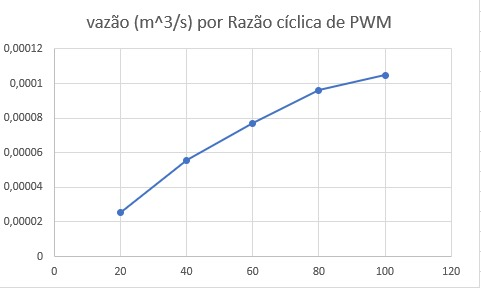
\includegraphics[scale=1]{imagens/graf0.jpeg}
    \end{center}
    \label{fig:graf0}
    \par Fonte: Dos autores
\end{figure}

A partir da linearização do gráfico foi estimado o valor da constante K em 0,0009027.
Para obtenção da área de saída do tanque, a, foi ligada a bomba em uma série de vazões conhecidas, e aguardado o sistema se estabilizar. Então, através da equação de Bernoulli, é calculada a área efetiva como $4.037088288e-5 m^2$.

Por fim, as alturas foram estimadas de maneira arbitrária, pois já que a importância dela para a equação de transferência é a precisão da linearização, desde que as alturas estejam bem distribuídas, espera-se um resultado adequado.

\subsection{Identificação por método Smith}

\subsubsection{Obtenção dos dados em malha aberta}
\hspace{11mm}O primeiro passo do método Smith requer que sejam coletados os dados da planta em malha aberta reagindo a um sinal de entrada degrau.

Como o sinal de razão cíclica de PWM aplicado não ativou a bomba com menos de 20\%, a metodologia seguida para aplicação de sinal foi de estabilizar o sistema em uma vazão de entrada constante, e então aumentar o sinal em um valor fixo. Os sinais foram aplicados da seguinte forma: de 20\% a 30\%, de 30\% a 40\%, de 40\% a 50\% e de 50\% a 60\% da razão cíclica de PWM formando assim quatro conjuntos de dados para uso do método Smith, que podem ser visto na imagem \ref{fig:graf}.

\begin{figure}[H]
    \centering\footnotesize
    \caption{Gráfico para calculo da constante K}
    \begin{center}
        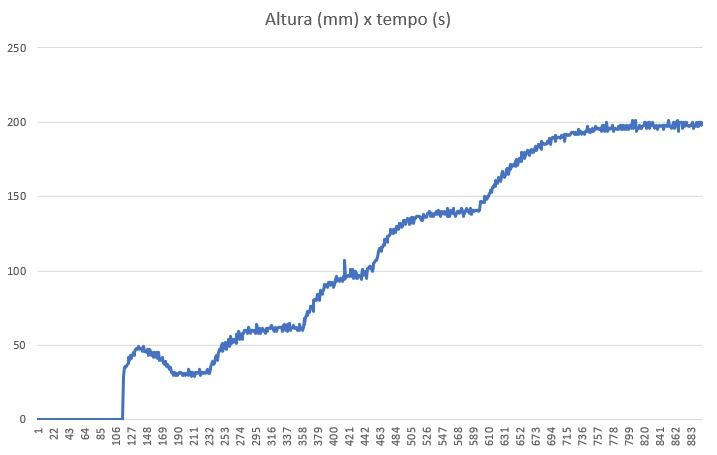
\includegraphics[scale=0.5]{imagens/grafico1.jpeg}
    \end{center}
    \label{fig:graf}
    \par Fonte: Dos autores
\end{figure}

\subsubsection{Aproximação da função Transferência}
\hspace{11mm}Para a aproximação da função de transferência aplicando o método Smith, foi utilizada uma rotina de Python, primeiramente os dados foram lidos e separado nos períodos correspondentes a cada conjunto:

\lstinputlisting[label=programa2, firstline=7, lastline=39, caption=Parse de dados]{codigos/identification.py}

Após isso foram aplicadas operações em todos os conjuntos simultaneamente, salvando os dados calculados no dicionário correspondente de cada conjunto. Iniciando pela transposição dos valores do gráfico, reduzindo o valor de todos os pontos baseado no menor valor do conjunto:
\lstinputlisting[label=programa3, firstline=58, lastline=61, caption=Transposição de valores]{codigos/identification.py}

Então foram calculadas a diferença da altura máxima para a primeira altura, $\Delta_h$:

\lstinputlisting[label=programa4, firstline=64, lastline=68, caption=Calculo Delta h]{codigos/identification.py}
    
Foi calculada a constante K e os tempos utilizados para o método de Smith:


\lstinputlisting[label=programa5, firstline=71, lastline=87, caption=Constante K e tempos utilizados]{codigos/identification.py}


Com estes dados foram obtidos as constantes da equação 2.1, tau e teta:

\lstinputlisting[label=programa6, firstline=90, lastline=100, caption=Calculo Tau e Theta]{codigos/identification.py}


E por fim foi calculada a função de transferência estimada para a planta:

\lstinputlisting[label=programa2, firstline=110, lastline=115, caption=Calculo Função transferência]{codigos/identification.py}

%\chapter{Resultados}
%\lettrine[lines=3]{}{} 
\chapter{Conclusão}

As considerações finais formam a parte final (fechamento) do texto, sendo dito de forma resumida (1) o que foi desenvolvido no presente trabalho e quais os resultados do mesmo, (2) o que se pôde concluir após o desenvolvimento bem como as principais contribuições do trabalho, e (3) perspectivas para o desenvolvimento de trabalhos futuros. O texto referente às considerações finais do autor deve salientar a extensão e os resultados da contribuição do trabalho e os argumentos utilizados estar baseados em dados comprovados e fundamentados nos resultados e na discussão do texto, contendo deduções lógicas correspondentes aos objetivos do trabalho, propostos inicialmente.

Antes de ir para as Referências, devo dizer que para obtê-las, você deve abrir o arquivo referencias.bib, neste arquivo estão as referências no formato \textit{BibTex}. Para que as citações apareçam no seu trabalho você deve:
\begin{itemize}
	\item pesquisar sobre o livro que você quer citar no site \textit{scholar.google.com.br}.
	\item colocar o nome do título do livro o qual você procura.
\end{itemize}

%referencias



% ----------------------------------------------------------
% ELEMENTOS PÓS-TEXTUAIS
% ----------------------------------------------------------
\postextual
\Spacing{1.5}
% -----------------------------------------------------------------------------
% Referencias Bibliograficas
% -----------------------------------------------------------------------------
%\bibliography{referencias}

% ----------------------------------------------------------
% Apêndices
% ----------------------------------------------------------

%% ---
% Inicia os apêndices
% ---
\begin{apendicesenv}
    
    % ----------------------------------------------------------
    \chapter{Primeiro apêndice}
    % ----------------------------------------------------------
    
    Os apêndices são textos ou documentos elaborados pelo autor, a fim de complementar sua argumentação, sem prejuízo da unidade nuclear do trabalho.
    
\end{apendicesenv}
%% Anexos
% ----------------------------------------------------------

% ---
% Inicia os anexos
% ---
\begin{anexosenv}

% ---
\chapter{Primeiro anexo.}
% ---

Os anexos são textos ou documentos não elaborados pelo autor, que servem de fundamentação, comprovação e ilustração.

\end{anexosenv}

\end{document}